% LuaLaTeX

\documentclass[a4paper, twoside, 12pt]{article}
\usepackage[latin]{babel} 
%\usepackage[landscape, left=3cm, right=1.5cm, top=2cm, bottom=1cm]{geometry} % okraje stranky
\usepackage[landscape, a4paper, mag=1166, truedimen, left=2cm, right=1.5cm, top=1.6cm, bottom=0.95cm]{geometry} % okraje stranky

\usepackage{fontspec}
\setmainfont[FeatureFile={junicode.fea}, Ligatures={Common, TeX}, RawFeature=+fixi]{Junicode}
%\setmainfont{Junicode}

% shortcut for Junicode without ligatures (for the Czech texts)
\newfontfamily\nlfont[FeatureFile={junicode.fea}, Ligatures={Common, TeX}, RawFeature=+fixi]{Junicode}

% Hebrew font:
% http://scripts.sil.org/cms/scripts/page.php?site_id=nrsi&id=SILHebrUnic2
\newfontfamily\hebfont[Scale=1]{Ezra SIL}

\usepackage{multicol}
\usepackage{color}
\usepackage{lettrine}
\usepackage{fancyhdr}

% usual packages loading:
\usepackage{luatextra}
\usepackage{graphicx} % support the \includegraphics command and options
\usepackage{gregoriotex} % for gregorio score inclusion
\usepackage{gregoriosyms}
\usepackage{wrapfig} % figures wrapped by the text
\usepackage{parcolumns}
\usepackage[contents={},opacity=1,scale=1,color=black]{background}
\usepackage{tikzpagenodes}
\usepackage{calc}
\usepackage{longtable}
\usetikzlibrary{calc}

\setlength{\headheight}{14.5pt}

% Commands used to produce a typical "Conventus" booklet

\newenvironment{titulusOfficii}{\begin{center}}{\end{center}}
\newcommand{\dies}[1]{#1

}
\newcommand{\nomenFesti}[1]{\textbf{\Large #1}

}
\newcommand{\celebratio}[1]{#1

}

\newcommand{\hora}[1]{%
\vspace{0.5cm}{\large \textbf{#1}}

\fancyhead[LE]{\thepage\ / #1}
\fancyhead[RO]{#1 / \thepage}
\addcontentsline{toc}{subsection}{#1}
}

% larger unit than a hora
\newcommand{\divisio}[1]{%
\begin{center}
{\Large \textsc{#1}}
\end{center}
\fancyhead[CO,CE]{#1}
\addcontentsline{toc}{section}{#1}
}

% a part of a hora, larger than pars
\newcommand{\subhora}[1]{
\begin{center}
{\large \textit{#1}}
\end{center}
%\fancyhead[CO,CE]{#1}
\addcontentsline{toc}{subsubsection}{#1}
}

% rubricated inline text
\newcommand{\rubricatum}[1]{\textit{#1}}

% standalone rubric
\newcommand{\rubrica}[1]{\vspace{3mm}\rubricatum{#1}}

\newcommand{\notitia}[1]{\textcolor{red}{#1}}

\newcommand{\scriptura}[1]{\hfill \small\textit{#1}}

\newcommand{\translatioCantus}[1]{\vspace{1mm}%
{\noindent\footnotesize \nlfont{#1}}}

% pruznejsi varianta nasledujiciho - umoznuje nastavit sirku sloupce
% s prekladem
\newcommand{\psalmusEtTranslatioB}[3]{
  \vspace{0.5cm}
  \begin{parcolumns}[colwidths={2=#3}, nofirstindent=true]{2}
    \colchunk{
      \input{#1}
    }

    \colchunk{
      \vspace{-0.5cm}
      {\footnotesize \nlfont
        \input{#2}
      }
    }
  \end{parcolumns}
}

\newcommand{\psalmusEtTranslatio}[2]{
  \psalmusEtTranslatioB{#1}{#2}{8.5cm}
}


\newcommand{\canticumMagnificatEtTranslatio}[1]{
  \psalmusEtTranslatioB{#1}{temporalia/extra-adventum-vespers/magnificat-boh.tex}{12cm}
}
\newcommand{\canticumBenedictusEtTranslatio}[1]{
  \psalmusEtTranslatioB{#1}{temporalia/extra-adventum-laudes/benedictus-boh.tex}{10.5cm}
}

% volne misto nad antifonami, kam si zpevaci dokresli neumy
\newcommand{\hicSuntNeumae}{\vspace{0.5cm}}

% prepinani mista mezi notovymi osnovami: pro neumovane a neneumovane zpevy
\newcommand{\cantusCumNeumis}{
  \setgrefactor{17}
  \global\advance\grespaceabovelines by 5mm%
}
\newcommand{\cantusSineNeumas}{
  \setgrefactor{17}
  \global\advance\grespaceabovelines by -5mm%
}

% znaky k umisteni nad inicialu zpevu
\newcommand{\superInitialam}[1]{\gresetfirstlineaboveinitial{\small {\textbf{#1}}}{\small {\textbf{#1}}}}

% pars officii, i.e. "oratio", ...
\newcommand{\pars}[1]{\textbf{#1}}

\newenvironment{psalmus}{
  \setlength{\parindent}{0pt}
  \setlength{\parskip}{5pt}
}{
  \setlength{\parindent}{10pt}
  \setlength{\parskip}{10pt}
}

%%%% Prejmenovat na latinske:
\newcommand{\nadpisZalmu}[1]{
  \hspace{2cm}\textbf{#1}\vspace{2mm}%
  \nopagebreak%

}

% mode, score, translation
\newcommand{\antiphona}[3]{%
\hicSuntNeumae
\superInitialam{#1}
\includescore{#2}

#3
}
 % Often used macros
%%%% Preklady jednotlivych zpevu (nektere se opakuji, a je dobre mit je
% vsechny na jedne hromade)

\newcommand{\trOratioAnteOfficium}{\translatioCantus{Otevři, Pane, má ústa, abych chválil tvé svaté jméno.
Očisti mé srdce od všech marnivých, zvrácených a~jiných myšlenek, osvěť rozum, rozněť cit,
abych mohl důstojně, soustředěně a~zbožně recitovat a~vysloužil si být
vyslyšen před tváří tvé velebnosti. Skrze Krista…}}

\newcommand{\trOratioPostOfficium}{\translatioCantus{\textit{Následující modlitbu
opatřil pro ty, kdo ji zbožně vyřknou po hodinkách, zesnulý papež Lev X.
odpustky za hříchy vzniklé při konání hodinek z~lidské křehkosti. Říká se
vkleče.}
Svatosvaté a~nerozdílné Trojici, ukřižovanému lidství našeho Pána Ježíše
Krista, přeblažené a~přeslavné plodné neporušenosti vždy Panny Marie
i~souhrnu všech svatých buď ode všeho stvoření věčná chvála, čest a~sláva, nám
pak buď dáno odpuštění všech hříchů, po nekonečné věky věků. Amen.}}

% HOURS ---

\newcommand{\trAntI}{\translatioCantus{Jasné narození slavné Panny Marie,
z pokolení (dosl. ze semene) Abrahámova, vzešlé z kmene Judova, z rodu Davidova.}}
\newcommand{\trAntII}{\translatioCantus{Dnes je Narození svaté Panny 
Marie, jejíž předrahý život osvěcuje všechny církve.}}

\newcommand{\trAntIII}{\translatioCantus{Maria, jež vzešla 
z královského rodu, září; myslí i duchem ji zbožně prosíme, aby 
nám pomáhala svými přímluvami.}}

\newcommand{\trAntIV}{\translatioCantus{Srdcem i duchem pějme Kristu 
k slávě o této svaté slavnosti vznešené Rodičky Boží Marie.}}

\newcommand{\trAntV}{\translatioCantus{Příjemně \notitia{?} 
oslavujme Narození blahoslavené Marie,
aby se ona za nás přimlouvala u Pána Ježíše Krista.}}

\newcommand{\trCapituli}{\translatioCantus{Před věky, na počátku mě stvořil, potrvám věčně. Ve svatém Stanu jsem před ním konala službu.}}

\newcommand{\trRespVesp}{\translatioCantus{Buď zdráva, Maria,
plná milosti: \grestar{} Pán s tebou. \Vbardot{} Požehnaná jsi mezi ženami,
a požehnaný plod života (ve smyslu lůna, břicha) tvého.}}

\newcommand{\trVersus}{\translatioCantus{\Vbardot{} Dnes je Narození svaté Panny Marie. \Rbardot{} Jejíž předrahý život osvěcuje všechny církve.}}

\newcommand{\trAntMagnificatI}{\translatioCantus{Konejme památku
veledůstojného narození slavné Panny Marie,
jíž se dostalo mateřské důstojnosti bez ztráty panenské cudnosti.}}

% Tento preklad je vice nez nejisty a ani alternativy, ktere jsem
% videl, me nepresvedcily...
\newcommand{\trAntBenedictus}{\translatioCantus{Slavnostně slavme 
dnešní narození Marie, vždy Panny a Rodičky Boží: v něm se objevuje
vysokost trůnu (totiž Marie, trůnu Božího Syna), aleluja.}}

\newcommand{\trAntMagnificatII}{\translatioCantus{Tvé narození,
Bohorodičko Panno, vyhlásilo radost celému světu:
z tebe totiž vzešlo Slunce spravedlnosti, Kristus, náš Bůh:
jenž zrušil kletbu a dal nám požehnání: přemohl smrt a dal nám život věčný.}}

\newcommand{\trOrationis}{\translatioCantus{Prosíme tě, Bože, 
uděl svým služebníkům dar nebeské milosti,
aby těm, jimž slehnutím blahoslavené Panny vyvstal počátek spásy, 
slavnost k poctě jejího narození přinesla
rozhojnění pokoje.
Skrze tvého Syna, našeho Pána Ježíše Krista, který s tebou žije a kraluje,
Bůh, v jednotě Ducha svatého po všechny věky věků.}}

\newcommand{\trFideliumAnimae}{\translatioCantus{\Vbardot{} Duše věrných ať pro
milosrdenství Boží odpočívají v~pokoji. \Rbardot{} Amen.}}

% Completorium

\newcommand{\trJubeDomne}{\translatioCantus{Rač, pane, požehnat.}}

\newcommand{\trComplBenedictio}{\translatioCantus{Pokojnou noc a~svatou smrt
nechť nám dopřeje všemohoucí Pán. \Rbardot{} Amen.}}

\newcommand{\trComplLectioBr}{\translatioCantus{Buďte střízliví, bděte.
Váš protivník Ďábel obchází jako lev řvoucí a~hledá, koho by pohltil.
Postavte se proti němu pevní ve víře.  Ale ty, Pane, smiluj se nad námi.
\Rbardot{} Bohu díky.}}

\newcommand{\trComplAntI}{\translatioCantus{Rač se smilovati nade mnou,
Hospodine, a vyslyš mou modlitbu.}}

\newcommand{\trComplCapituli}{\translatioCantus{Jsi přece, Hospodine,
uprostřed nás a~jmenujeme se po tobě.  Neopouštěj nás, Pane, náš Bože.}}

\newcommand{\trRespCompl}{\translatioCantus{Do tvých rukou, Pane, \grestar{}
poroučím svého ducha. \Vbardot{} Ty mne zachráníš, Pane, Bože věrný.}}

\newcommand{\trComplVersus}{\translatioCantus{\Vbardot{} Střez mne jako zřítelnici oka,
aleluja. \Rbardot{} Ve stínu svých křídel uschovej mne, aleluja.}}

\newcommand{\trAntSalvaNos}{\translatioCantus{Ochraňuj nás, Pane, když
bdíme, a~buď s~námi, když spíme, ať bdíme s~Kristem a~odpočíváme v~pokoji.}}

\newcommand{\trComplOrationis}{\translatioCantus{Zavítej, prosíme, Pane, sem
do našeho příbytku a~daleko od něj zažeň všechny úklady nepřítele. Ať tu
bydlí tví svatí andělé a~tvoje požehnání buď nad ním stále. Skrze…}}

\newcommand{\trSalveRegina}{\translatioCantus{Zdrávas Královno, matko
milosrdenství, živote, sladkosti a naděje naše, buď zdráva!
K tobě voláme, vyhnaní synové Evy,
k tobě vzdycháme, lkajíce a plačíce
v tomto slzavém údolí.
A proto, orodovnice naše,
obrať k nám své milosrdné oči
a Ježíše, požehnaný plod života svého,
nám po tomto putování ukaž,
ó milostivá, ó přívětivá,
ó přesladká, Panno Maria!}}

\newcommand{\trOraProNobis}{\translatioCantus{\Vbardot{} 
Oroduj za nás, svatá Boží Rodičko,
\Rbardot{} aby nám Kristus dal účast na svých zaslíbeních.}}

% Matutinum

\newcommand{\trMatInvitatorium}{\translatioCantus{}}

\newcommand{\trMatVeniteA}{\translatioCantus{Pojďte, chvalme s~radostí Pána,
s~jásotem slavme Boha, svou spásu; předstupme před tvář jeho s~díky, písně plesu pějme jemu.}}

\newcommand{\trMatVeniteB}{\translatioCantus{Neboť Bůh veliký jest Hospodin, a~král nade všecky bohy.
Jsouť v~jeho ruce všecky hlubiny země, temena hor jsou majetek jeho.}}

\newcommand{\trMatVeniteC}{\translatioCantus{Jehoť jest moře, neb on je učinil; i~souš
je dílo jeho rukou. Pojďme, klanějme se, padněme, klekněme před Pánem, svým
tvůrcem. Jeť on Pán, náš Bůh, a~my jsme lid, jejž on vodí a~ovce, jež pase.}}

\newcommand{\trMatVeniteD}{\translatioCantus{Kéž byste poslechli dnes hlasu jeho:
,,Nezatvrzujte svých srdcí jak v~Hádce, jak v~Pokušení na poušti, kde vaši otcové pokoušeli mne,
zkoušeli mne, ač vídali skutky mé.``}}

\newcommand{\trMatVeniteE}{\translatioCantus{Čtyřicet roků mrzel jsem se na to pokolení
a~řekl jsem: ,,Lid je to myslí stále bloudící``! Oni však nechtěli znáti mé cesty, takže jsem
přisáhl ve svém hněvu: ,,Nedojdou odpočinku mého!\mbox{}``}}

\newcommand{\trMatAntI}{\translatioCantus{}}

\newcommand{\trMatAntII}{\translatioCantus{}}

\newcommand{\trMatAntIII}{\translatioCantus{}}

\newcommand{\trMatVersusI}{\translatioCantus{}}

\newcommand{\trMatAbsolutioI}{\translatioCantus{Vyslyš Pane Ježíši Kriste
prosby svých služebníků \gredagger{} a~smiluj se nad námi, \grestar{} jenž
s~Otcem a~Duchem…}}

\newcommand{\trMatBenedictioI}{\translatioCantus{Rač, pane, požehnat.
Věčný Otec nám stále žehnej. \Rbardot{} Amen.}}

\newcommand{\trMatLecI}{\translatioCantus{Kéž by mě zulíbal polibky svých úst. 
Tvé milování je nad víno lahodnější;
vybraně voní tvé voňavky;
rozlévající se olej je tvé jméno,
proto tě dívky milují.
Strhni mě za sebou, poběžme!
Král mě uvedl do svých komnat;
budeš nám radostí a jásotem.
Víc než víno oslavíme tvé milování;
věru po právu jsi milován!
Snědá jsem, a přece krásná, jeruzalémské dcery,
jako stany kedarské,
jako šalmské závěsy.
}}

\newcommand{\trMatRespI}{\translatioCantus{}}

\newcommand{\trMatBenedictioII}{\translatioCantus{Rač, pane, požehnat.
Jednorozený Boží Syn nám žehnej \grestar{} a nám pomáhej. \Rbardot{} Amen.}}

\newcommand{\trMatLecII}{\translatioCantus{Nehleďte na mou osmahlou pleť:
to mě slunce ožehlo.
Synové mé matky se na mne rozzlobili,
poslali mě hlídat vinice.
A svou vinici, tu jsem nehlídala!
Pověz mi tedy, ty, jehož miluje mé srdce:
kam zavedeš své stádo pást,
kde ho necháš za poledne odpočívat?
Abych už nebloudila jako tulačka
poblíž stád druhů tvých.
Nevíš-li to, nejrásnější z žen,
jdi po stopách stáda
a kůzlata svá zaveď, ať se pasou
poblíž obydlí pastýřů.
Ke své klisně zapřažené do vozu faraonova
tebe, mé milá, přirovnávám.
Stále krásné jsou tvé líce s náušnicemi
i tvé hrdlo v náhrdelnících.}}

\newcommand{\trMatRespII}{\translatioCantus{}}

\newcommand{\trMatBenedictioIII}{\translatioCantus{Rač, pane, požehnat.
Milost Ducha Svatého ať osvítí nám smysly \grestar{} i srdce. \Rbardot{} Amen.}}

\newcommand{\trMatLecIII}{\translatioCantus{Zhotovíme ti zlaté náušnice
a kuličky ze stříbra.
Když král stoluje,
vydechuje můj nard svou vůni.
Můj milý je polštářek s myrhou,
jenž mi odpočívá mezi ňadry.
Můj milý je hrozen šáchoru
ve vinicích v Engadi.
Jak jsi krásná, milá moje,
jak jsi krásná!
Tvé oči jsou holubice.
Jak jsi krásný, můj milý,
jak líbezný!
Naše lože je samá zeleň.
Trámoví našeho domu je z cedru,
naše ostění z cypřiše.}}

\newcommand{\trMatRespIII}{\translatioCantus{}}

\newcommand{\trMatAntIV}{\translatioCantus{}}

\newcommand{\trMatAntV}{\translatioCantus{}}

\newcommand{\trMatAntVI}{\translatioCantus{}}

\newcommand{\trMatVersusII}{\translatioCantus{}}

\newcommand{\trMatAbsolutioII}{\translatioCantus{
Tvá milost a laskavost nechť nám pomáhá, jenž žiješ a vládneš s Otcem a Svatým Duchem na věky věků.}}

\newcommand{\trMatBenedictioIV}{\translatioCantus{Rač, pane, požehnat.
Bůh Otec všemohoucí, \grestar{} buď k nám milostivý a odpouštějící. \Rbardot{} Amen.}}

\newcommand{\trMatLecIV}{\translatioCantus{}}

\newcommand{\trMatRespIV}{\translatioCantus{}}

\newcommand{\trMatBenedictioV}{\translatioCantus{}}

\newcommand{\trMatLecV}{\translatioCantus{}}

\newcommand{\trMatRespV}{\translatioCantus{}}

\newcommand{\trMatBenedictioVI}{\translatioCantus{Rač, pane, požehnat.
Bůh rozněť v nás oheň své lásky. \Rbardot{} Amen.}}

\newcommand{\trMatLecVI}{\translatioCantus{}}

\newcommand{\trMatRespVI}{\translatioCantus{}}

\newcommand{\trMatAntVII}{\translatioCantus{}}

\newcommand{\trMatAntVIII}{\translatioCantus{}}

\newcommand{\trMatAntIX}{\translatioCantus{}}

\newcommand{\trMatVersusIII}{\translatioCantus{}}

\newcommand{\trMatAbsolutioIII}{\translatioCantus{Z okovů našich hříchů,
\grestar{} vysvoboď nás všemohoucí a milosrdný Pán. \Rbardot{} Amen.}}

\newcommand{\trMatBenedictioVII}{\translatioCantus{Rač, pane, požehnat.
Čtení evangelia nechť je nám \grestar{} spásou a ochranou. \Rbardot{} Amen.}}

\newcommand{\trMatLecVIIa}{\translatioCantus{
  Rodokmen Ježíše Krista, syna Davidova, syna Abrahámova:
  Abrahám zplodil Izáka,
  Izák zplodil Jakuba.}}

\newcommand{\trMatLecVIIb}{\translatioCantus{}}

\newcommand{\trMatRespVII}{\translatioCantus{}}

\newcommand{\trMatBenedictioVIII}{\translatioCantus{Rač, pane, požehnat.
\Rbardot{} Amen.}}

\newcommand{\trMatLecVIII}{\translatioCantus{}}

\newcommand{\trMatRespVIII}{\translatioCantus{}}

\newcommand{\trMatBenedictioIX}{\translatioCantus{Rač, pane, požehnat.
Do společnosti občanů nebes \grestar{} ať nás dovede král andělů.
\Rbardot{} Amen.}}

\newcommand{\trMatLecIX}{\translatioCantus{}}

% from the Czech Liturgia horarum
\newcommand{\trTeDeum}{\begin{translatioMulticol}{3}

Bože, tebe chválíme, 
tebe, Pane, velebíme.

Tebe, věčný Otče, 
oslavuje celá země.

Všichni andělé, 
cherubové i~serafové,

všechny mocné nebeské zástupy 
bez ustání volají:

Svatý, Svatý, Svatý, 
Pán, Bůh zástupů.

Plná jsou nebesa i~země 
tvé vznešené slávy.

Oslavuje tě 
sbor tvých apoštolů,

chválí tě 
velký počet proroků,

vydává o~tobě svědectví 
zástup mučedníků;

a~po celém světě 
vyznává tě tvá církev:

neskonale velebný, 
všemohoucí Otče,

úctyhodný Synu Boží, 
pravý a~jediný,

božský Utěšiteli, 
Duchu svatý.

Kriste, Králi slávy, 
tys od věků Syn Boha Otce;

abys člověka vykoupil, 
stal ses člověkem a~narodil ses z~Panny;

zlomil jsi osten smrti 
a~otevřel věřícím nebe;

sedíš po Otcově pravici 
a~máš účast na jeho slávě.

Věříme, že přijdeš soudit, 

a~proto tě prosíme:
přispěj na pomoc svým služebníkům, 
vždyť jsi je vykoupil svou předrahou krví;

dej, ať se radují s~tvými svatými 
ve věčné slávě.

Zachraň, Pane, svůj lid, žehnej svému dědictví, 
veď ho a~stále pozvedej.

Každý den tě budeme velebit 
a~chválit tvé jméno po všechny věky.

Pomáhej nám i~dnes, 
ať se nedostaneme do područí hříchu.

Smiluj se nad námi, Pane, 
smiluj se nad námi.

Ať spočine na nás tvé milosrdenství, 
jak doufáme v~tebe.

Pane, k~tobě se utíkáme, 
ať nejsme zahanbeni na věky. 
\end{translatioMulticol}}

\newcommand{\trMatEvangelium}{\translatioCantus{
  Rodokmen Ježíše Krista, syna Davidova, syna Abrahámova:
  Abrahám zplodil Izáka,
  Izák zplodil Jakuba,
  Jakub zplodil Judu a jeho bratry,
  Juda zplodil Farese a Zaru z Tamary,
  Fares zplodil Esroma,
  Esrom zplodil Arama,
  Aram zplodil Aminadaba,
  Aminadab zplodil Naasona,
  Naason zplodil Salmona,
  Salmon zplodil Boaze z Rahaby,
  Boaz zplodil Jobeda z Rut,
  Jobed zplodil Jessea,
  Jesse zplodil krále Davida.
  David zplodil Šalomouna z Uriášovy ženy,
  Šalomoun zplodil Roboama,
  Roboam zplodil Abiu,
  Abia zplodil Asu,
  Asa zplodil Josafata,
  Josafat zplodil Jorama,
  Joram zplodil Oziáše,
  Oziáš zplodil Joatama,
  Joatam zplodil Achaze,
  Achaz zplodil Ezechiáše,
  Ezechiáš zplodil Manasesa,
  Manases zplodil Amona,
  Amon zplodil Josiáše,
  Josiáš zplodil Jechoniáše a jeho bratry;
  tehdy došlo k odvlečení do Babylonu.
  Po odvlečení do Babylonu:
  Jechoniáš zplodil Salatiela,
  Salatiel zplodil Zorobabela,
  Zorobabel zplodil Abiuda,
  Abiud zplodil Eljakima,
  Eljakim zplodil Azora,
  Ator zplodil Sadoka,
  Sadok zplodil Achima,
  Achim zplodil Eliuda,
  Eliud zplodil Eleazara,
  Eleatar zplodil Matana,
  Matan zplodil Jakuba,
  Jakub zplodil Josefa, manžela Marie,
  z níž se narodil Ježíš, který se nazývá Kristus.}}

\newcommand{\trTeDecetLaus}{\translatioCantus{Tobě chvála, Tobě zpěvy, Tobě
sláva, Bohu Otci i~Synu i~Svatému Duchu, na věky věků. \Rbardot{} Amen.}}

% MASS ---

\newcommand{\trIntroitus}{\translatioCantus{Radujme se všichni
v Pánu, slavíce svátek ke cti Panny Marie: z něj se radují andělé
a spoluchválí Božího Syna. \textit{\color{red}Žl.} Má ústa vydala dobré slovo,
přednáším svá díla králi.}}

\newcommand{\trGraduale}{\translatioCantus{Požehnaná a ctihodná jsi,
Panno Maria: nedotčená (co do panenství) jsi byla shledána matkou
Spasitele. \Vbardot{} Panno Boží Rodičko, ten, jehož nepojme ani celý svět,
se uzavřel do tvých útrob, když se stal člověkem.}}

\newcommand{\trAlleluia}{\translatioCantus{Aleluja. \Vbardot{} Skvělá slavnost
slavné Panny Marie, z pokolení (dosl. ze semene) Abrahámova, vzešlé z kmene 
Judova, z rodu Davidova.}}

\newcommand{\trOffertorium}{\translatioCantus{Blažená jsi, Panno Maria,
tys nosila Stvořitele všeho; porodila jsi toho, který tě utvořil,
a na věky zůstáváš Pannou.}}

\newcommand{\trCommunio}{\translatioCantus{Budou mě blahoslavit
všechna pokolení, protože mi učinil veliké věci ten, který je mocný.}}

% LITTLE HOURS ---

\newcommand{\trVersusTertia}{\translatioCantus{\Vbardot{} \Rbardot{}}}

\newcommand{\trCapituliEtSic}{\translatioCantus{
Tak jsem se usadila na Sionu a v milovaném městě jsem nalezla odpočinek,
v Jeruzalémě vykonávám svou moc.
Zakořenila jsem u lidu plného slývy, na panství Páně, v jeho dědictví.}}

\newcommand{\trVersusSexta}{\translatioCantus{\Vbardot{} \Rbardot{}}}

\newcommand{\trCapituliInPlateis}{\translatioCantus{
Na planině jako skořicovník a akant jsem vydávala vůni, jako vybraná myrha
jsem voněla.}}

\newcommand{\trVersusNona}{\translatioCantus{\Vbardot{} \Rbardot{}}}
 % Czech translations of the proper texts

\newcommand{\annusEditionis}{2015}

\def\hebinitial#1{%
\leavevmode{\newbox\hebbox\setbox\hebbox\hbox{\hebfont{#1}\hskip 1mm}\kern -\wd\hebbox\hbox{\hebfont{#1}\hskip 1mm}}%
}

%%%% Vicekrat opakovane kousky

\newcommand{\anteOrationem}{
  \rubrica{Ante Orationem, cantatur a Superiore:}

  \pars{Supplicatio Litaniæ.}

  \cuminitiali{}{temporalia/supplicatiolitaniae.gtex}

  \pars{Oratio Dominica.}

  \cuminitiali{}{temporalia/oratiodominica.gtex}

  \rubrica{Deinde dicitur ab Hebdomadario:}

  \cuminitiali{}{temporalia/dominusvobiscum-solemnis.gtex}

  \rubrica{In choro monialium loco Dominus vobiscum dicitur:}

  \sineinitiali{temporalia/domineexaudi.gtex}
}

\newcommand{\tuAutem}{
  \vfill

  \sineinitiali{temporalia/tuautem.gtex}
}

\setlength{\columnsep}{30pt} % prostor mezi sloupci

%%%%%%%%%%%%%%%%%%%%%%%%%%%%%%%%%%%%%%%%%%%%%%%%%%%%%%%%%%%%%%%%%%%%%%%%%%%%%%%%%%%%%%%%%%%%%%%%%%%%%%%%%%%%%
\begin{document}

% Here we set the space around the initial.
% Please report to http://home.gna.org/gregorio/gregoriotex/details for more details and options
\grechangedim{afterinitialshift}{2.2mm}{scalable}
\grechangedim{beforeinitialshift}{2.2mm}{scalable}

\grechangedim{interwordspacetext}{0.32 cm plus 0.15 cm minus 0.05 cm}{scalable}%
\grechangedim{annotationraise}{-0.2cm}{scalable}

% Here we set the initial font. Change 38 if you want a bigger initial.
% Emit the initials in red.
\grechangestyle{initial}{\color{red}\fontsize{38}{38}\selectfont}

\pagestyle{empty}

%%%% Titulni stranka
\begin{titulusOfficii}
\nomenFesti{Dominica II Adventus.}
\celebratio{II Classis. Semiduplex.}
\end{titulusOfficii}

% graphic
\vfill
\begin{center}
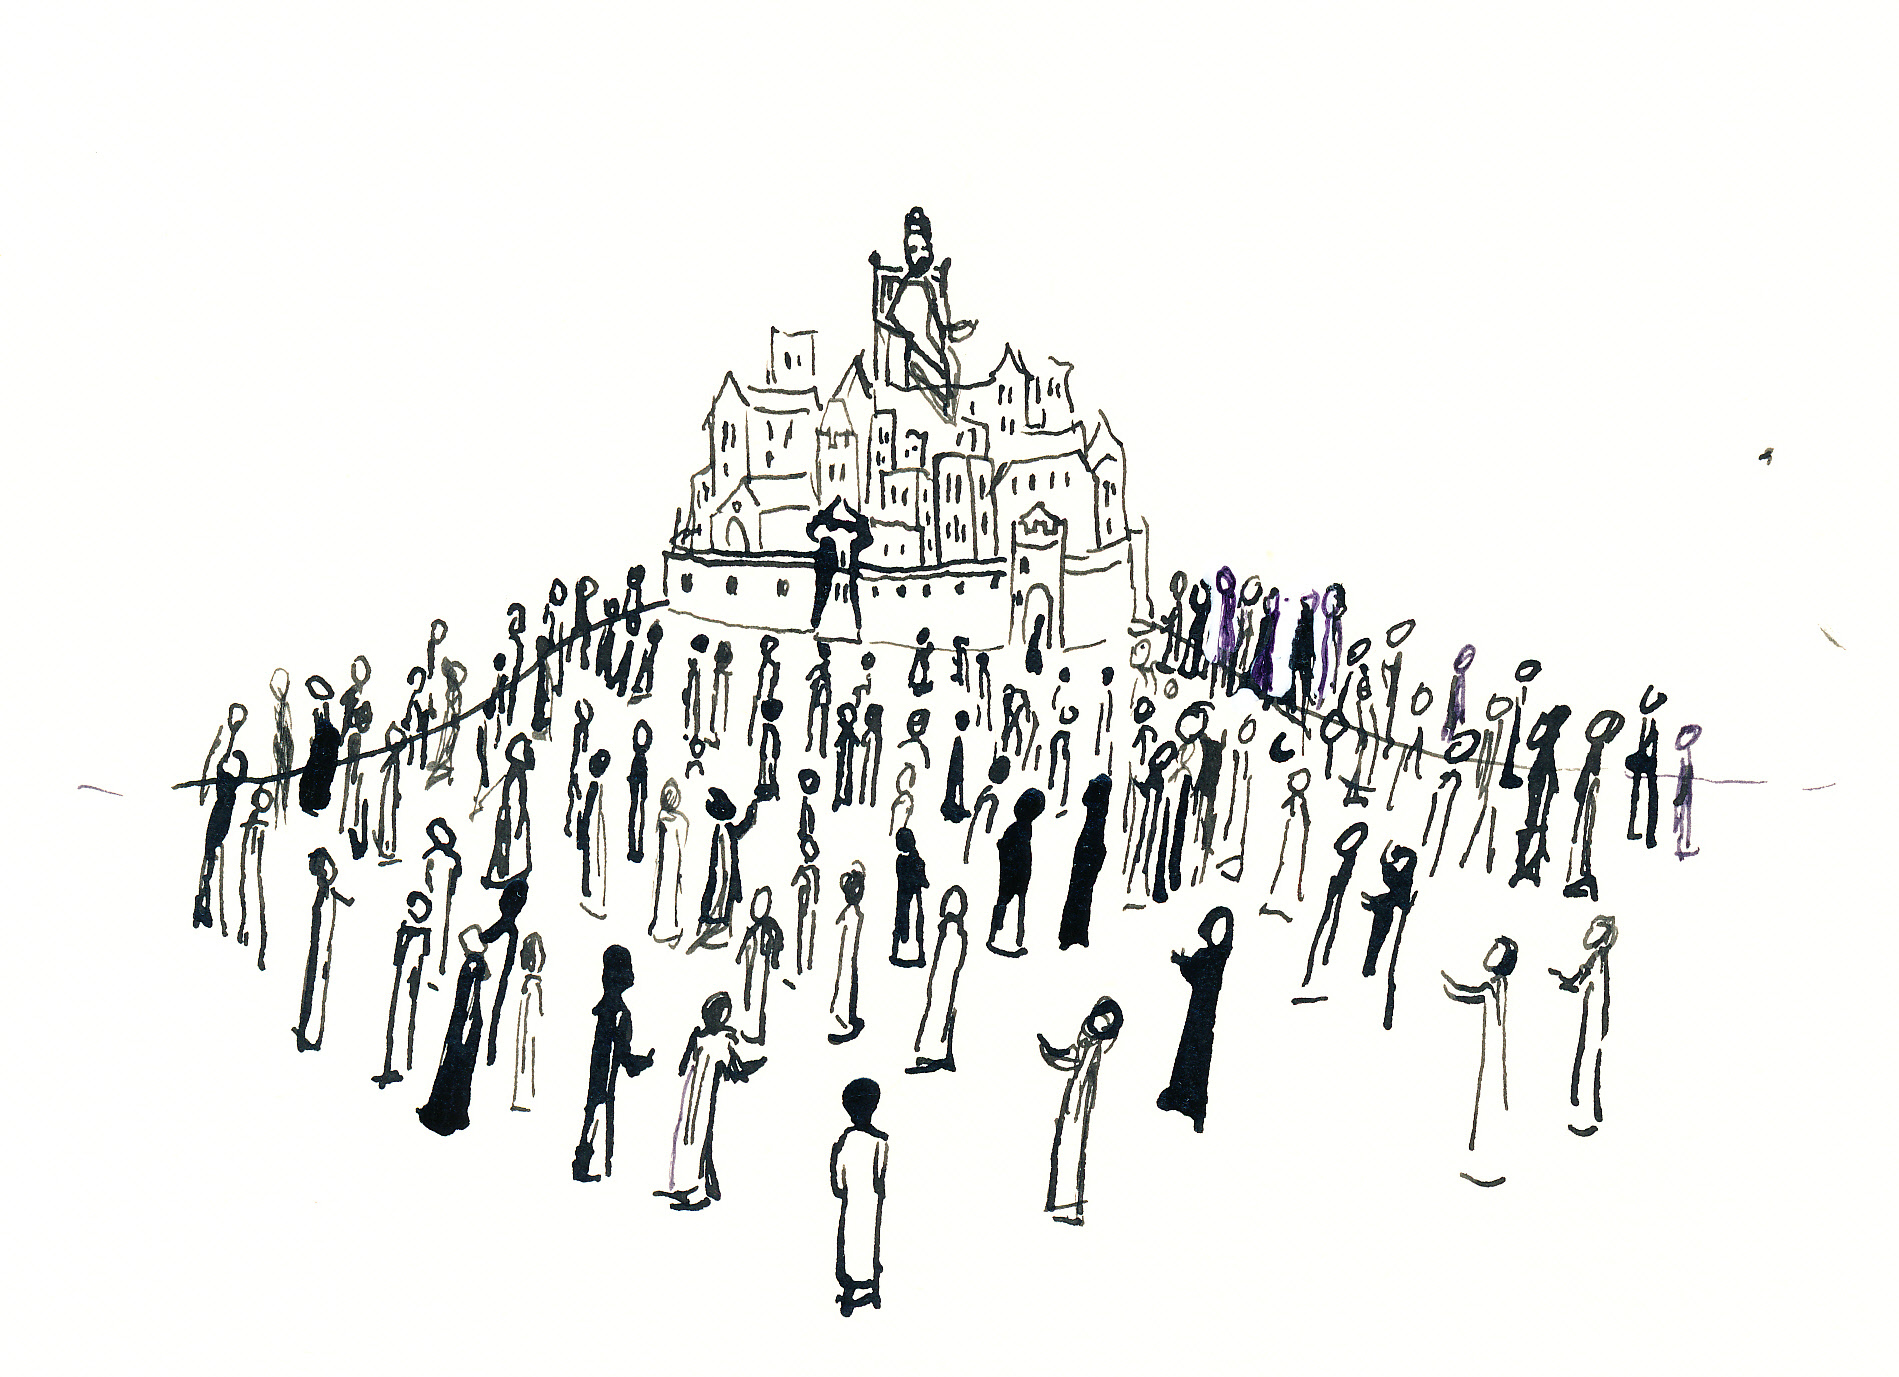
\includegraphics[width=15cm]{imagines/imago_Sion.jpg}
\end{center}

\vfill

\begin{center}
Ad usum et secundum consuetudines chori \guillemotright Conventus Choralis\guillemotleft.

Editio Sancti Wolfgangi \annusEditionis
\end{center}

\pagebreak

\renewcommand{\headrulewidth}{0pt} % no horiz. rule at the header
\fancyhf{}
\pagestyle{fancy}

\pars{Léctio sancti Evangélii secúndum Matthǽum.} \scriptura{Mt. 11, 2-10}

\textusEtTranslatio{
  In illo témpore:
  Cum audísset Ioánnes in vínculis ópera Christi, mittens duos de discípulis suis,
  ait illi: Tu es, qui ventúrus es, an álium exspectámus?
  Et respóndens Iesus ait illis:
  Eúntes renuntiáte Ioánni quæ audístis et vidístis.
  Cæci vident, claudi ámbulant, leprósi mundántur, surdi áudiunt, mórtui resúrgunt, páuperes evangelizántur:
  et beátus est, qui non fúerit scandalizátus in me.
  Illis autem abeúntibus, cæpit Iesus dícere ad turbas de Ioánne: Quid exístis in desértum vidére?
  arúndinem vento agitátam?
  Sed quid exístis vidére?
  hóminem móllibus vestítum?
  Ecce qui móllibus vestiúntur, in dómibus regum sunt.
  Sed quid exístis vidére prophétam?
  Etiam dico vobis et plus quam prophétam.
  Hic est enim, de quo scriptum est:
  Ecce ego mitto ángelum meum ante fáciem tuam,
  qui preparábit viam tuam ante te.
}{\trMatEvangelium}{10cm}

\vspace{2cm}

\cantusSineNeumas

\pars{Antiphona}

\vspace{-0.3cm}

{
\grechangedim{interwordspacetext}{0.10 cm plus 0.15 cm minus 0.05 cm}{scalable}%
\antiphona{I}{temporalia/ant-rorate.gtex}
\grechangedim{interwordspacetext}{0.32 cm plus 0.15 cm minus 0.05 cm}{scalable}%
}

\begin{translatioMulticol}{3}
Dej rosu, nebe nad námi,\\
ať z oblak skane spása.\\
\\
Odlož hněv svůj, ó Pane náš\\
a zapomeň už na naše nepravosti.\\
Hle, tvé svaté město je pouští,\\
opuštěný je Sión, Jeruzalém je liduprázdný,\\
to místo tobě zasvěcené, dům tvé slávy,\\
kde k chvále tvé zpívali otcové naši.\columnbreak

Pro hříchy své stali jsme se lidem nečistým\\
a odpadli jsme jako zvadlé listí.\\
Jako vichr nás uchvátily naše viny,\\
když jsi před námi ukryl svou tvář\\
a vydal nás napospas nepravosti naši.\\

Pohlédni, Pane, na ponížení lidu svého,\\
ať příjde ten, jenž přijít má.\\
Pošli Beránka, ať vládne zemi,\\
od Skály na poušti až k hoře siónské dcery.\\
Ať on sám sejme jho poroby naší.\columnbreak

Přijmi útěchu, přijmi útěchu, můj lide drahý,\\
neboť blízko je tvoje spása.\\
Proč se stále trápíš v úzkostech,\\
proč tě bolest svírá?\\
Zachráním tě, neboj se, doufej!\\
Vždyť já to jsem, já Hospodin, Pán a Bůh tvůj,\\
izraelův Svatý a Spása tvoje.
\end{translatioMulticol}


\vfill
\pagebreak

\pars{Oratio ante divinum Officium.}

\lettrine{{\color{red}A}}{peri,} Dómine, os meum ad benedicéndum nomen sanctum tuum:
munda quoque cor meum ab ómnibus vanis, pervérsis, et aliénis
cogitatiónibus:
intelléctum illúmina, afféctum inflámma,
ut digne, atténte ac devóte hoc Offícium recitáre váleam,
et exaudíri mérear ante conspéctum Divínæ Maiestátis tuæ.
Per Christum, Dominum nostrum.
\Rbardot{} Amen.

Dómine, in unióne illíus divínæ intentiónis,
qua ipse in terris laudes Deo persolvísti,
has tibi Horas \rubricatum{(vel \textnormal{hanc tibi Horam})} persólvo.

\trOratioAnteOfficium

\vfill

\pars{Oratio post divinum Officium.}

\rubrica{
  Orationem sequentem devote post Officium recitantibus
  Leo Papa X. defectus, et culpas in eo persolvendo ex humana
  fragilitate contractas, indulsit, et dicitur flexis genibus.
}

\lettrine{{\color{red}S}}{acrosánctæ} et indivíduæ Trinitáti,
crucifíxi Dómini nostri Iesu Christi humanitáti,
beatíssimæ et gloriosíssimæ sempérque Vírginis Maríæ
fecúndæ integritáti, 
et ómnium Sanctórum universitáti
sit sempitérna laus, honor, virtus et glória
ab omni creatúra,
nobísque remíssio ómnium peccatórum,
per infiníta sǽcula sæculórum.
\Rbardot{} Amen.

\noindent \Vbardot{} Beáta víscera Maríæ Virginis, quæ portavérunt
ætérni Patris Fílium.\\
\Rbardot{} Et beáta úbera, quæ lactavérunt Christum Dominum.

\rubrica{Et dicitur secreto \textnormal{Pater noster.} et \textnormal{Ave María.}}

\trOratioPostOfficium

\vfill

\hora{Sabbato ad Vesperas.} %%%%%%%%%%%%%%%%%%%%%%%%%%%%%%%%%%%%%%%%%%%%%%%%%%%%%
\sideThumbs{I. Vesperæ}

\cantusSineNeumas

{
\grechangedim{interwordspacetext}{0.28 cm plus 0.15 cm minus 0.05 cm}{scalable}%
\cuminitiali{}{temporalia/deusinadiutorium-alter.gtex}
\grechangedim{interwordspacetext}{0.32 cm plus 0.15 cm minus 0.05 cm}{scalable}%
}

\vfill
\pagebreak

\cantusCumNeumis

\pars{Psalmus 1.} \scriptura{Cf. Dn. 3, 17.18; Mc. 13, 26; \textbf{H23}}

\vspace{-0.5cm}

\antiphona{I g}{temporalia/ant1.gtex}

\trAntI

\cantusSineNeumas

\scriptura{Ps. 143, 1-8}

\initiumpsalmi{temporalia/ps143i-initium-i-g-auto.gtex}

\psalmusEtTranslatioT{temporalia/ps143i-comb.tex}{10cm}

\vfill
\pagebreak

\pars{Psalmus 2.} \scriptura{Is. 26, 1.2; \textbf{H24}}

\vspace{-0.5cm}

\antiphona{VII d}{temporalia/ant2.gtex}

\trAntII

\scriptura{Ps. 143, 9-15}

\initiumpsalmi{temporalia/ps143ii-initium-vii-d-auto.gtex}

\vspace{-0.2cm}

\psalmusEtTranslatioT{temporalia/ps143ii-comb.tex}{10cm}

\vfill
\pagebreak

\pars{Psalmus 3.} \scriptura{Hab. 2, 3; \textbf{H24}}

\vspace{-0.5cm}

\antiphona{VII a}{temporalia/ant3.gtex}

\trAntIII

\scriptura{Ps. 144, 1-7}

\initiumpsalmi{temporalia/ps144i_vii-initium-vii-a-auto.gtex}

\psalmusEtTranslatioT{temporalia/ps144i_vii-comb.tex}{10cm}

\vfill
\pagebreak

\pars{Psalmus 4.} \scriptura{Cf. Is. 55, 12; \textbf{H24}}

\vspace{-0.5cm}

\antiphona{I f}{temporalia/ant4.gtex}

\trAntIV

\scriptura{Ps. 144, 8-13}

\initiumpsalmi{temporalia/ps144viii_xiii-initium-i-f-auto.gtex}

\psalmusEtTranslatioT{temporalia/ps144viii_xiii-comb.tex}{10cm}

\vfill
\pagebreak

\pars{Psalmus 5.} \scriptura{\textbf{H24}}

\vspace{-0.5cm}

\antiphona{III a}{temporalia/ant5.gtex}

\trAntV

\scriptura{Ps. 144, 14-21}

\initiumpsalmi{temporalia/ps144xiv_xxi-initium-iii-a-auto.gtex}

\psalmusEtTranslatioT{temporalia/ps144xiv_xxi-comb.tex}{10cm}

\vfill
\pagebreak

\raggedcolumns

% Capitulum. %%%
\cantusSineNeumas

\pars{Capitulum.} \scriptura{Rom. 15, 4}

\cuminitiali{}{temporalia/capitulum-FratresQuaecumque.gtex}

% preklad Jeruz. bible
\trCapituli

\vfill
\pars{Responsorium breve.} \scriptura{Ps. 84, 8; \textbf{H20}}

{
\grechangedim{interwordspacetext}{0.28 cm plus 0.15 cm minus 0.05 cm}{scalable}%
\cuminitiali{IV}{temporalia/resp-vesp.gtex}
\grechangedim{interwordspacetext}{0.32 cm plus 0.15 cm minus 0.05 cm}{scalable}%
}

\trRespVesp

\vfill
\pagebreak

% Hymnus. %%%
\pars{Hymnus.}

{
\grechangedim{interwordspacetext}{0.17 cm plus 0.15 cm minus 0.05 cm}{scalable}%
\cuminitiali{IV}{temporalia/hym-ConditorAlme.gtex}
\grechangedim{interwordspacetext}{0.32 cm plus 0.15 cm minus 0.05 cm}{scalable}%
}
\begin{translatioMulticol}{3}
Štědrý nebes stvořiteli\\
Věčný osvítiteli\\
Kriste vykupiteli\\
prosby vyslyš věrných milý.\\
\\
Nad zánikem věku v~smrti\\
smiloval ses, milý choti\\
a~světu spásy lačnému\\
lék jsi přinesl vinnému.\columnbreak

Když se večer světa chýlí,\\
vyšels jako ženich milý\\
z~domu matky, panny čestné,\\
z~její komnaty milostné.\\
\\
Mocí tvojí velmi silnou\\
kolena se k~zemi ohnou\\
a~nebe, země tvorové\\
se poddávají vůli tvé.\columnbreak

Jenž přicházíš věku soudce,\\
prosíme tě světovládce,\\
uchovej nás v~našem čase\\
před úkladnou ranou zhoubce.\\
\\
Chválu, sílu, čest a~slávu,\\
Bohu Otci, jeho Synu,\\
Duchu také rady svaté\\
vzdej na věky věků světe.\\
Amen.
\end{translatioMulticol}


\vspace{-0.4cm}

\pars{Versus.} \scriptura{Is. 45, 8}

% Versus. %%%
\sineinitiali{temporalia/versus-rorate.gtex}
\noindent \trVersusVesp

\vfill
\pagebreak

\cantusCumNeumis

\pars{Canticum B. Mariæ V.} \scriptura{\textbf{H21}}

\vspace{-0.5cm}

{
\grechangedim{interwordspacetext}{0.24 cm plus 0.15 cm minus 0.05 cm}{scalable}%
\antiphona{VII a}{temporalia/ant-magn-vesp1.gtex}
\grechangedim{interwordspacetext}{0.32 cm plus 0.15 cm minus 0.05 cm}{scalable}%
}

\trAntMagnificatI

\vfill

\scriptura{Lc. 1, 46-55}

\cantusSineNeumas
\initiumpsalmi{temporalia/magnificat-initium-vii-a.gtex}

\psalmusEtTranslatioT{temporalia/magnificat-comb.tex}{10.3cm}

\vfill
\pagebreak

\anteOrationem

\pagebreak

% Oratio. %%%
\pars{Oratio.}

\cuminitiali{}{temporalia/oratio.gtex}
\trOrationis

\vspace{1cm}
\rubrica{Hebdomadarius dicit iterum Dominus vobiscum. Postea cantatur a cantore:}
\vspace{2mm}

\cuminitiali{IV}{temporalia/benedicamus-dominica-advequad.gtex}

\vfill
\pagebreak

\hora{Ad Completorium.} %%%%%%%%%%%%%%%%%%%%%%%%%%%%%%%%%%%%%%%%%%%%%%%%%%%%%%%%%%
\sideThumbs{{\scriptsize{}Completorium}}

\rubrica{Lector petit benedictionem, dicens:}

\cuminitiali{}{temporalia/jubedomnebenedicere.gtex}

\trJubeDomne

\vfill

\pars{Benedictio.}

\cuminitiali{}{temporalia/benedictio-noctemquietam.gtex}

\trComplBenedictio

\vfill

\pars{Lectio brevis.} \scriptura{1Ptr. 5, 8-9}

\cuminitiali{}{temporalia/lectiobrevis-fratressobrii.gtex}

\trComplLectioBr

\vfill

\noindent \Vbardot{} Adiutórium nostrum in nómine Dómini. \Rbardot{} Qui fecit cælum, et terram.

\vfill

\noindent Pater noster \rubricatum{quod dicitur totum secreto.}

\vfill
\pagebreak

\pars{Confessio.}

\noindent Confíteor Deo omnipoténti, beátæ Maríæ semper Vírgini, beáto
Michaéli Archángelo, beáto Ioánni Baptístæ, sanctis Apóstolis Petro
et Paulo, ómnibus Sanctis, et vobis fratres: quia peccávi nimis cogitatióne,
verbo et ópere: mea culpa, mea culpa, mea máxima culpa.
Ídeo precor beátam Maríam semper Vírginem, beátum Michaélum
Archángelum, beátum Ioánnem Baptístam, sanctos Apóstolos Petrum
et Paulum, omnes Sanctos, et vos fratres, oráre pro me ad Dóminum
Deum nostrum.

\vfill

\noindent \Vbardot{} Misereátur nostri omnípotens Deus, et, dimíssis peccátis nostris, perdúcat
nos ad vitam ætérnam. \Rbardot{} Amen.

\vfill

\noindent \Vbardot{} Indulgéntiam, absolutiónem et remissiónem peccatórum nostrórum tríbuat nobis
omnípotens et miséricors Dóminus. \Rbardot{} Amen.

\vfill

\rubrica{Et facta absolutione dicitur:}

\sineinitiali{temporalia/convertenosdeus.gtex}

\vfill

\cuminitiali{}{temporalia/deusinadiutorium-communis.gtex}

\vfill
\pagebreak

\pars{Psalmus 1.} \scriptura{Cf. Ps. 4, 2}

\vspace{-0.5cm}

\antiphona{VIII G}{temporalia/ant-miserere.gtex}

\trComplAntI

\scriptura{Ps. 4}

\initiumpsalmi{temporalia/ps4-initium-viii-G-auto.gtex}

\psalmusEtTranslatioT{temporalia/ps4-comb.tex}{10cm}

\vfill
\pagebreak

\pars{Psalmus 2.} \scriptura{Ps. 90}

\psalmusEtTranslatioT{temporalia/ps90-comb.tex}{10cm}

\pagebreak

\pars{Psalmus 3.} \scriptura{Ps. 133}

\psalmusEtTranslatioT{temporalia/ps133-comb.tex}{10cm}

\vfill

\antiphona{VIII G}{temporalia/ant-miserere.gtex}

\vfill

\pars{Hymnus.}

\antiphona{IV}{temporalia/hym-TeLucis.gtex}
\begin{translatioMulticol}{3}
Než světlo zhasne prosíme\\
Tebe tvůrce všech pokorně,\\
abys nám ve své milosti\\
byl ochranou a~pomocí.\columnbreak

Ať vzdáleny jsou od nás sny\\
a~těžké noční přízraky.\\
Zdrť našeho nepřítele,\\
těla poskvrn ať ujdeme.\columnbreak

Tobě buď sláva, Ježíši,\\
národům že ses projevil,\\
Otci i~Duchu života\\
po věkoucí věky světa.\\
Amen.
\end{translatioMulticol}


\pagebreak

\pars{Capitulum.} \scriptura{Ier. 14, 9}

\cuminitiali{}{temporalia/capitulum-tuautem.gtex}

% preklad Jeruz. bible
\trComplCapituli

\vfill

\pars{Responsorium breve.} \scriptura{Ps. 30, 6}

\cuminitiali{IV}{temporalia/resp-inmanus.gtex}

\trRespCompl
\vfill

\pars{Versus.} \scriptura{Ps. 16, 8}

{
\grechangedim{interwordspacetext}{0.24 cm plus 0.15 cm minus 0.05 cm}{scalable}%
\sineinitiali{temporalia/versus-custodi.gtex}
\grechangedim{interwordspacetext}{0.32 cm plus 0.15 cm minus 0.05 cm}{scalable}%
}

\noindent \trComplVersus

\vfill
\pagebreak

\cantusCumNeumis

\pars{Canticum Simeonis.}

\vspace{-0.5cm}

{
\grechangedim{interwordspacetext}{0.30 cm plus 0.15 cm minus 0.05 cm}{scalable}%
\antiphona{III a}{temporalia/ant-salvanos-antiquo.gtex}
\grechangedim{interwordspacetext}{0.32 cm plus 0.15 cm minus 0.05 cm}{scalable}%
}

\trAntSalvaNos

\scriptura{Lc. 2, 29-32}

\initiumpsalmi{temporalia/nuncdimittis-initium-iii-a-auto.gtex}

\psalmusEtTranslatioT{temporalia/nuncdimittis-comb.tex}{10cm}

\vfill
\pagebreak

\pars{Oratio.}

\cantusSineNeumas

\cuminitiali{}{temporalia/oratio-visita.gtex}

\trComplOrationis

\vfill

\sineinitiali{temporalia/domineexaudi.gtex}

\vfill

\sineinitiali{temporalia/benedicamus-minor.gtex}

\vfill

\pars{Benedictio.}

\noindent Benedícat et custódiat nos omnípotens et miséricors Dóminus, \gredagger{}
Pater, et Fílius, et Spíritus Sanctus. \Rbardot{} Amen.

\vfill
\pagebreak

\pars{Antiphona finalis B. M. V.}

\antiphona{V}{temporalia/an_alma_redemptoris_mater.gtex}

\trAlmaRedemptoris

\vfill

\sineinitiali{temporalia/versus-angelus.gtex}

\trAngelusDomini

\vfill
\pagebreak

\pars{Oratio.}

\cuminitiali{}{temporalia/oratio-AlmaRedemptorisAdvent.gtex}
\trComplOrationisGratiam

\vspace{0.5cm}

\sineinitiali{temporalia/divinumauxilium.gtex}

\trComplDivinum

\vfill
\pagebreak

\hora{Ad Matutinum.} %%%%%%%%%%%%%%%%%%%%%%%%%%%%%%%%%%%%%%%%%%%%%%%%%%%%%%%%%%
\sideThumbs{Matutinum}

\vspace{2mm}

\cuminitiali{}{temporalia/dominelabiamea.gtex}

\vspace{2mm}

\pars{Invitatorium.}

\vspace{-2mm}

\antiphona{V}{temporalia/matinv-RegemVenturum.gtex}

\trMatInvitatorium

\scriptura{Ps. 94 (Textus antiquus latinus); \textbf{H447}}

\vspace{-5mm}

\antiphona{V}{temporalia/venite5a.gtex}

\trMatVeniteA

\scriptura{Repetitur integrum Invitatorium.}

\antiphona{}{temporalia/venite5b.gtex}

\trMatVeniteB

\scriptura{Repetitur altera pars Invitatorii.}

\rubrica{In sequenti Psalmi versu, ad verba \textnormal{veníte, adorémus et procidámus ante Deum}, genuflectitur.}

\antiphona{}{temporalia/venite5c.gtex}

\trMatVeniteC

\scriptura{Repetitur integrum Invitatorium.}

\antiphona{}{temporalia/venite5d.gtex}

\trMatVeniteD

\scriptura{Repetitur altera pars Invitatorii.}

\vfill
\pagebreak

\antiphona{}{temporalia/venite5e.gtex}

\trMatVeniteE

\scriptura{Repetitur integrum Invitatorium.}

\antiphona{}{temporalia/venite5f.gtex}

\scriptura{Repetitur altera pars Invitatorii. Denique repetitur integrum Invitatorium.}

\antiphona{}{temporalia/matinv-RegemVenturum.gtex}

\vfill
\pagebreak

\pars{Hymnus.}

\vspace{-0.5cm}

{
\grechangedim{interwordspacetext}{0.30 cm plus 0.15 cm minus 0.05 cm}{scalable}%
\antiphona{VIII}{temporalia/hym-VerbumSupernum.gtex}
\grechangedim{interwordspacetext}{0.32 cm plus 0.15 cm minus 0.05 cm}{scalable}%
}
{
\vspace{0.5cm}
\setlength{\columnsep}{0pt} % prostor mezi sloupci
\begin{translatioMulticol}{5}
Nebeské Slovo, Syn ty jsi\\
a světlo z Otce prýštící,\\
jenž zrozen, jdeš zachránit svět,\\
když naplnil se časů věk.\columnbreak

Už teď nám duši rozjasni\\
a plamen lásky zapal v ní,\\
ať srdce vlády zbavené\\
nebeská rozkoš naplní.\columnbreak

Aby, až soudce na trůnu\\
ohni zlé bude vydávat\\
a ty, kdo toho hodni jsou,\\
milý hlas v nebe povolá,\columnbreak

zmatku temnot ať vydáni\\
nejsme, ni v stravu plamenů,\\
leč na tvář Boha pohledět\\
smíme a těšit se v nebesích.\columnbreak

Otci společně se Synem,\\
a Tobě, Duše přesvatý,\\
sláva, jež vždycky trvala,\\
stejná budiž i na věky.\\
Amen.
\end{translatioMulticol}

\setlength{\columnsep}{30pt} % prostor mezi sloupci
}

\vfill
\pagebreak

\subhora{In I. Nocturno}

\pars{Psalmus 1.} \scriptura{Cf. Zach. 9, 9}

\antiphona{I g}{temporalia/matant1.gtex}

\trMatAntI

\scriptura{Ps. 1}

\initiumpsalmi{temporalia/ps1-initium-i-g-auto.gtex}

\psalmusEtTranslatioT{temporalia/ps1-comb.tex}{10cm}

\vfill
\pagebreak

\pars{Psalmus 2.} \scriptura{Is. 35, 3.4}

\antiphona{II d}{temporalia/matant2.gtex}

\trMatAntII

\scriptura{Ps. 2}

\initiumpsalmi{temporalia/ps2-initium-ii-D-auto.gtex}

\psalmusEtTranslatioT{temporalia/ps2-comb.tex}{10cm}

\vfill
\pagebreak

\pars{Psalmus 3.} \scriptura{Cf. Is. 66, 10}

\antiphona{III a}{temporalia/matant3.gtex}

\trMatAntIII

\scriptura{Ps. 3}

\initiumpsalmi{temporalia/ps3-initium-iii-a-auto.gtex}

\psalmusEtTranslatioT{temporalia/ps3-comb.tex}{10cm}

\vfill
\pagebreak

\pars{Versus.} \scriptura{Ps. 49, 2.3}

\sineinitiali{temporalia/versus-exsion.gtex}

\noindent \trMatVersusI

\vfill

\sineinitiali{temporalia/oratiodominica-mat.gtex}

\vfill

\pars{Absolutio.}

\cuminitiali{}{temporalia/absolutio-exaudi.gtex}

\trMatAbsolutioI

\vfill
\pagebreak

\cuminitiali{}{temporalia/benedictio-solemn-benedictione.gtex}

\trMatBenedictioI

\vfill

\cuminitiali{}{temporalia/tonus-lectionis-solemnis.gtex}

\vfill

% De Isaia Prophéta.
\pars{Lectio I.} \scriptura{Is. 11, 1-4}

\noindent De Isaia \textit{Pro}phéta.

\textusEtTranslatio{
  Et egrediétur virga de rádice Iesse,
  et flos de rádice eius as\textbf{cén}det;~\gredagger{}
  et requiéscet super eum spíritus Dómini:
  spíritus sapiéntiæ et \textit{in}telléctus,~\grestar{}
  spíritus consílii et forti\textbf{tú}dinis,~\gredagger{}
  spíritus sciéntiæ et \textit{pi}etátis;~\grestar{}
  Et replébit eum spíritus timó\textit{ris} Dómini.
  Non secúndum visiónem oculórum iudicábit
  neque secúndum audítum áurium \textbf{ár}guet;~\gredagger{}
  Sed iudicábit in iustíti\textit{a} páuperes,~\grestar{}
  et árguet in æquitáte pro mansué\textit{tis} terræ.
}{\trMatLecI}{10cm}

\tuAutem

\vfill
\pagebreak

\pars{Responsorium 1.} \scriptura{\Rbar{} Mch. 4, 8.9 \Vbar{} Cantor; \textbf{H21}}

\responsorium{IV}{temporalia/matresp1.gtex}{\trMatRespI}

\vfill
\pagebreak

\cuminitiali{}{temporalia/benedictio-solemn-unigenitus.gtex}

\trMatBenedictioII

\vfill

\pars{Lectio II.} \scriptura{Is. 11, 4-7}

\textusEtTranslatio{
  Et percútiet terram virga \textit{o}ris sui,~\grestar{}
  et spíritu labiórum suórum interfíci\textit{et} ímpium.
  Et erit iustítia cíngulum lum\textit{bó}rum eius,~\grestar{}
  et fides cinctórium re\textit{num} eius.
  Habitábit lupus cum agno,
  et pardus cum hædo accu\textbf{bá}bit;~\gredagger{}
  vítulus, et leo, et ovis, simul \textit{mo}rabúntur,~\grestar{}
  et puer párvulus miná\textit{bit} eos.
  Vítulus et ursus pas\textbf{cén}tur,~\gredagger{}
  simul requiéscent cátu\textit{li} eórum;~\grestar{}
  et leo quasi bos cóme\textit{det} páleas.
}{\trMatLecII}{10cm}

\tuAutem

\vfill
\pagebreak

\pars{Responsorium 2.} \scriptura{\Rbar{} Zach. 14, 5.7-9 \Vbar{} Is. 40, 10; \textbf{H22}}

\responsorium{V}{temporalia/matresp2.gtex}{\trMatRespII}

\vfill
\pagebreak

\cuminitiali{}{temporalia/benedictio-solemn-spiritus.gtex}

\trMatBenedictioIII

\vfill

\pars{Lectio III.} \scriptura{Is. 11, 8-10}

\textusEtTranslatio{
  Et delectábitur infans ab úbere
  super forá\textit{mi}ne áspidis;~\grestar{}
  et in cavérna réguli
  qui ablactátus fúerit manum su\textit{am} mittet.
  Non nocébunt et non occídent
  in univérso monte sancto \textbf{me}o,~\gredagger{}
  quia repléta est terra scién\textit{ti}a Dómini,~\grestar{}
  sicut aquæ maris ope\textit{ri}éntes.
  In die illa radix Iesse,
  qui stat in signum popu\textbf{ló}rum,~\gredagger{}
  ipsum gentes de\textit{pre}cabúntur,~\grestar{}
  et erit sepúlcrum eius glo\textit{ri}ósum.
}{\trMatLecIII}{10cm}

\tuAutem

\vfill
\pagebreak

\pars{Responsorium 3.} \scriptura{\Rbar{} Cantor \Vbar{} Is. 40, 10; \textbf{H22}}

\responsorium{I}{temporalia/matresp3.gtex}{\trMatRespIII}

\vfill
\pagebreak

\subhora{In II. Nocturno}

\pars{Psalmus 4.} \scriptura{Cf. Lam. 4, 21}

{
\grechangedim{interwordspacetext}{0.20 cm plus 0.15 cm minus 0.05 cm}{scalable}%
\antiphona{IV e}{temporalia/matant4.gtex}
\grechangedim{interwordspacetext}{0.32 cm plus 0.15 cm minus 0.05 cm}{scalable}%
}

\trMatAntIV

\scriptura{Ps. 8}

\initiumpsalmi{temporalia/ps8-initium-iv-E-auto.gtex}

\psalmusEtTranslatioT{temporalia/ps8-comb.tex}{10cm}

\vfill
\pagebreak

\pars{Psalmus 5.}

\antiphona{V a}{temporalia/matant5.gtex}

\trMatAntV

\scriptura{Ps. 9, 2-11}

\initiumpsalmi{temporalia/ps9ii_xi-initium-v-a-auto.gtex}

\psalmusEtTranslatioT{temporalia/ps9ii_xi-comb.tex}{10cm}

\vfill
\pagebreak

\pars{Psalmus 6.} \scriptura{Apc. 22, 12}

\antiphona{VI f}{temporalia/matant6.gtex}

\trMatAntVI

\scriptura{Ps. 9, 12-21}

\initiumpsalmi{temporalia/ps9xii_xxi-initium-vi-F-auto.gtex}

\psalmusEtTranslatioT{temporalia/ps9xii_xxi-comb.tex}{10cm}

\vfill
\pagebreak

\pars{Versus.} \scriptura{Is. 16, 1}

\sineinitiali{temporalia/versus-emitte.gtex}

\noindent \trMatVersusII

\vfill

\sineinitiali{temporalia/oratiodominica-mat.gtex}

\vfill

\pars{Absolutio.}

\cuminitiali{}{temporalia/absolutio-ipsius.gtex}

\trMatAbsolutioII

\vfill
\pagebreak

\cuminitiali{}{temporalia/benedictio-solemn-deus.gtex}

\trMatBenedictioIV

\vfill

% De Expositióne sancti Hierónymi Presbytéri in Isaíam Prophétam
\pars{Lectio IV.} \scriptura{Lib. 4. in cap. 11. Isaiæ.}

\noindent De Expositióne sancti Hierónymi Presbytéri in Isaíam \textit{Pro}phétam.

\textusEtTranslatio{
  Et egrediétur virga de rádi\textit{ce} Iesse.
  Usque ad princípium visiónis, vel pónderis Babylónis, quod vidit Isaías, fílius \textbf{A}mos,~\gredagger{}
  omnis hæc prophétia de Christo est: quam per partes vólumus \textit{ex}planáre,~\grestar{}
  ne simul propósita atque dissérta lectóris confúndat \textit{me}móriam.
  Virgam et florem de rádice Iesse ipsum Dóminum Iudǽi interpre\textbf{tán}tur:~\gredagger{}
  quod scílicet in virga regnán\textit{tis} poténtia,~\grestar{}
  in flore pulchritúdo \textit{mon}strétur.
}{\trMatLecIV}{10cm}

\tuAutem

\vfill
\pagebreak

\pars{Responsorium 4.} \scriptura{\Rbar{} Is. 43, 14.15 \Vbar{} Cantor; \textbf{H22}}

\responsorium{V}{temporalia/matresp4.gtex}{\trMatRespIV}

\vfill
\pagebreak

\cuminitiali{}{temporalia/benedictio-solemn-christus.gtex}

\trMatBenedictioV

\vfill

\pars{Lectio V.} \scriptura{Lib. 4. in cap. 11. Isaiæ.}

\textusEtTranslatio{
  Nam et sævítia Heródis volens primórdia suspécti sibi Regis exs\textbf{tín}guere,~\gredagger{}
  huic dispensatíoni nésciens serviébat: ut dum atróci intén\textit{tus} facínori,~\grestar{}
  ignótum sibi púerum indiscréta infántium cæde per\textbf{sé}quitur,~\gredagger{}
  annuntiátum cǽlitus dominatóris ortum insígnior ubíque fama \textit{lo}querétur:~\grestar{}
  quam promptiórem ad nar\textbf{rán}dum,~\gredagger{}
  diligentiorémque faciébat et supérnæ significati\textit{ó}nis nóvitas,~\grestar{}
  et cruentíssimi persecutóris \textit{im}píetas.
  Tunc autem étiam Ægýpto Salvátor il\textbf{lá}tus est,~\gredagger{}
  ut gens antíquis erró\textit{ri}bus dédita,~\grestar{}
  iam ad vicínam salútem per occúltam grátiam signa\textbf{ré}tur:~\gredagger{}
  et quæ nondum eiécerat ab ánimo super\textit{sti}tiónem,~\grestar{}
  iam hospítio recíperet ve\textit{ri}tátem.
}{\trMatLecV}{10cm}

\tuAutem

\vfill
\pagebreak

\pars{Responsorium 5.} \scriptura{\Rbar{} Is. 66, 13.14 \Vbar{} Is. 46, 13; \textbf{H22}}

\responsorium{VIII}{temporalia/matresp5.gtex}{\trMatRespV}

\vfill
\pagebreak

\cuminitiali{}{temporalia/benedictio-solemn-ignem.gtex}

\trMatBenedictioVI

\vfill

\pars{Lectio VI.} \scriptura{Lib. 4. in cap. 11. Isaiæ.}

\textusEtTranslatio{
  Agnoscámus ergo, dilec\textbf{tís}simi,~\gredagger{}
  in Magis adoratóribus Christi, vocatiónis nostræ fideí\textit{que} primítias:~\grestar{}
  et exsultántibus ánimis beátæ spei inítia ce\textit{leb}rémus.
  Exínde enim in ætérnam hereditátem cœ́pimus intro\textbf{í}re:~\gredagger{}
  exínde nobis Christum loquéntia Scripturárum arcána patué\textit{runt,} et \hbox{véritas,~\grestar{}}
  quam Iudæórum obcæcátio non récipit, ómnibus natiónibus lumen suum \textit{in}véxit.
  Honorétur ítaque a nobis sacratíssimus dies, in quo salútis nostræ Auctor ap\textbf{pá}ruit:~\gredagger{}
  et quem Magi infántem veneráti sunt \textit{in} cunábulis,~\grestar{}
  nos omnipoténtem adorémus \textit{in} cælis.
  Ac sicut illi de thesáuris suis mýsticas Dómino múnerum spécies obtu\textbf{lé}runt,~\gredagger{}
  ita et nos de cór\textit{di}bus nostris,~\grestar{}
  quæ Deo sunt digna, \textit{pro}mámus.
}{\trMatLecVI}{10cm}

\tuAutem

\vfill
\pagebreak

\pars{Responsorium 6.} \scriptura{\Rbar{} Ir. 31, 5-7 \Vbar{} Zach. 9, 9; \textbf{H23}}

\responsorium{VIII}{temporalia/matresp6.gtex}{\trMatRespVI}

\vfill
\pagebreak

\subhora{In III. Nocturno}

\pars{Psalmus 7.} \scriptura{Ambros. Expos. Evang. Lc. lib. 2}

\vspace{-0.2cm}

\antiphona{VII d}{temporalia/matant7.gtex}

\trMatAntVII \scriptura{Ps. 9, 22-32}

\initiumpsalmi{temporalia/ps9xxii_xxxii-initium-vii-d-auto.gtex}

\psalmusEtTranslatioT{temporalia/ps9xxii_xxxii-comb.tex}{10.5cm}

\antiphona{}{temporalia/matant7.gtex} % repeat the antiphon - new page

\vfill
\pagebreak

\pars{Psalmus 8.}

\antiphona{VIII g}{temporalia/matant8.gtex}

\trMatAntVIII

\scriptura{Ps. 9, 33-39}

\initiumpsalmi{temporalia/ps9xxxiii_xxxix-initium-viii-g-auto.gtex}

\psalmusEtTranslatioT{temporalia/ps9xxxiii_xxxix-comb.tex}{10cm}

\vfill
\pagebreak

\pars{Psalmus 9.}

\antiphona{IV e}{temporalia/matant9.gtex}

\trMatAntIX

\scriptura{Ps. 10}

\initiumpsalmi{temporalia/ps10-initium-iv-E-auto.gtex}

\psalmusEtTranslatioT{temporalia/ps10-comb.tex}{10cm}

\vfill
\pagebreak

\pars{Versus.} \scriptura{Cf. Mch. 1, 3}

\sineinitiali{temporalia/versus-egredietur.gtex}

\noindent \trMatVersusIII

\vfill

\sineinitiali{temporalia/oratiodominica-mat.gtex}

\vfill

\pars{Absolutio.}

\cuminitiali{}{temporalia/absolutio-avinculis.gtex}

\trMatAbsolutioIII

\vfill
\pagebreak

\cuminitiali{}{temporalia/benedictio-solemn-evangelica.gtex}

\trMatBenedictioVII

\vfill

% Léctio sancti Evangélii secúndum Matthǽum.
\pars{Lectio VII.} \scriptura{Mt. 11, 2-10}

\noindent Léctio sancti Evangélii secúndum \textit{Mat}thǽum.

\textusEtTranslatio{
  In illo tempóre: Cum audísset Ioánnes in vínculis ópera \textbf{Chris}ti,~\gredagger{}
  mittens duos de discí\textit{pu}lis suis,~\grestar{}
  ait illi: \textit{Tu} es qui ventúrus es, an álium ex\textit{spec}támus?
  \textit{Et} relíqua.
}{\trMatLecVIIa}{10cm}

% Homilía sancti Gregórii Papæ.
\scriptura{Homilia 6. in Evang. post init.}

\noindent Homilía sancti Gregóri\textit{i} Papæ.

\textusEtTranslatio{
  Visis tot signis tantís\textit{que} virtútibus,~\grestar{}
  non scandalizári quisque pótuit, sed ad\textit{mi}rári.
  Sed infidélium mens grave in illo scán\textit{da}lum pértulit,~\grestar{}
  cum eum post tot mirácula morién\textit{tem} vidit.
  Unde et Paulus \textbf{di}cit:~\gredagger{}
  Nos autem prædicámus Christum \textit{cru}cifíxum,~\grestar{}
  Iudǽis quidem scándalum, géntibus autem \textit{stul}títiam.
  Stultum quippe homínibus visum est, ut pro homínibus Auctor vitæ more\textbf{ré}tur:~\gredagger{}
  et inde contra eum homo scán\textit{da}lum sumpsit,~\grestar{}
  unde ei ámplius débitor fíe\textit{ri} débuit.
  Nam tanto Deus ab homínibus dígnius \textit{ho}norándus est,~\grestar{}
  quanto pro homínibus et indígna \textit{sus}cépit.
}{\trMatLecVIIb}{10cm}

\tuAutem

\vfill
\pagebreak

\pars{Responsorium 7.} \scriptura{\Rbar{} Cantor \Vbar{} Is. 16, 5; \textbf{H23}}

\responsorium{III}{temporalia/matresp7.gtex}{\trMatRespVII}

\vfill
\pagebreak

\cuminitiali{}{temporalia/benedictio-solemn-divinum.gtex}

\trMatBenedictioVIII

\vfill

\pars{Lectio VIII.} \scriptura{Homilia 6. in Evang. post init.}

\textusEtTranslatio{
  Quid est ergo \textbf{dí}cere:~\gredagger{}
  Beátus qui non fúerit scandali\textit{zá}tus in me;~\grestar{}
  nisi apérta \textit{vo}ce abiectiónem mortis suæ humilitatémque \textit{sig}náre?
  Ac si paténter \textbf{di}cat:~\gredagger{}
  Mira \textit{qui}dem fácio,~\grestar{}
  sed abiécta perpéti non \textit{de}dígnor.
  Quia ergo moriéndo te súbsequor, cavéndum valde est ho\textbf{mí}nibus,~\gredagger{}
  ne in me mor\textit{tem} despíciant,~\grestar{}
  qui signa ve\textit{ne}rántur.
}{\trMatLecVIII}{10cm}

\tuAutem

\vfill
\pagebreak

\pars{Responsorium 8.} \scriptura{\Rbar{} Cantor \Vbar{} Hab. 2, 3; \textbf{H34}}

\responsorium{II}{temporalia/matresp8.gtex}{\trMatRespVIII}

\vfill
\pagebreak

\cuminitiali{}{temporalia/benedictio-solemn-adsocietatem.gtex}

\trMatBenedictioIX

\vfill

\pars{Lectio IX.} \scriptura{Homilia 6. in Evang. post init.}

\textusEtTranslatio{
  Sed dimíssis Ioán\textit{nis} discípulis,~\grestar{}
  quid de eódem Ioánne turbis dicat, au\textit{di}ámus.
  Quid exístis \textit{in} desértum \textit{vi}dére?
  Arúndinem \textit{ven}to a\textit{gi}tátam?
  Quod vidélicet non \textit{as}seréndo,~\grestar{}
  sed negán\textit{do} íntulit.
  Arúndinem quippe mox ut au\textit{ra} contígerit,~\grestar{}
  in partem álteram \textit{in}fléctit.
  Et quid per arúndinem, \textit{ni}si carnális ánimus de\textit{sig}nátur?
  Qui mox ut favóre vel detractióne tángitur, \textit{sta}tim in partem quámlibet in\textit{cli}nátur?
}{\trMatLecIX}{10cm}

\tuAutem

\vfill
\pagebreak

\pars{Responsorium 9.} \scriptura{\Rbar{} Cantor \Vbar{} Is. 40, 10}

\responsorium{III}{temporalia/matresp9.gtex}{\trMatRespIX}

\vfill
\pagebreak

% Evangelium

\cuminitiali{}{temporalia/tonus-evangelii-b.gtex}

\vfill

\pars{Léctio san\textit{cti} Evangélii {\textnormal{\grestar{}}} secúndum Mat\textit{thǽ}um.} \scriptura{Mt. 11, 2-10}

\textusEtTranslatio{
  \textit{In} illo témpore:~\grestar{}
  Cum audísset Ioánnes in vínculis ópera Christi, mittens duos de \textit{dis}cípulis suis,~\grestar{}
  ait illi: \textit{Tu} es, qui ventúrus es, an álium ex\textit{spec}támus?
  Et respóndens Ie\textit{sus} ait illis:~\grestar{}
  Eúntes renuntiáte Ioánni quæ audístis et vi\textbf{dís}tis.
  Cæci vident, claudi ámbulant, leprósi mundántur, surdi áudiunt, mórtui resúrgunt, páuperes \textit{e}vangelizántur:~\grestar{}
  et beátus est, qui non fúerit scandalizátus \textbf{in} me.
  Illis autem abeúntibus, cæpit Iesus dícere ad turbas de Ioánne: \textit{Quid} exístis in desértum \textit{vi}dére?
  arúndinem \textit{ven}to a\textit{gi}tátam?
  Sed quid \textit{ex}ístis \textit{vi}dére?
  hóminem \textit{mól}libus \textit{ves}títum?
  Ecce qui móllibus vestiúntur, in dómibus \textbf{re}gum sunt.
  Sed quid \textit{ex}ístis vidére \textit{pro}phétam?
  Etiam dico vobis et plus quam pro\textbf{phé}tam.
  Hic est e\textit{nim}, de quo scriptum est:~\grestar{}
  Ecce ego mitto ángelum meum ante fáciem \textbf{tu}am,
  \textit{qui} preparábit viam tuam \textbf{an}te te.
}{\trMatEvangelium}{10cm}

\vfill
\cuminitiali{I}{temporalia/tedecetlaus.gtex}

\trTeDecetLaus

\vfill
\pagebreak

\sineinitiali{temporalia/domineexaudi.gtex}

\vfill

\pars{Oratio.}

\cuminitiali{}{temporalia/oratio.gtex}
\trOrationis

\vfill

\noindent \Vbardot{} Dómine, exáudi oratiónem meam.
\Rbardot{} Et clamor meus ad te véniat.

\vfill

% Nocturnale Romanum 2002, p. LXXVI Benedicamus Domino seems to match
% the one from Solemn Laudes.
\cuminitiali{V}{temporalia/benedicamus-solemnis-laud.gtex}

\vfill

\noindent \Vbardot{} Fidélium ánimæ per misericórdiam Dei requiéscant in pace.
\Rbardot{} Amen.

\trFideliumAnimae

\vfill
\pagebreak

\hora{Ad Laudes.} %%%%%%%%%%%%%%%%%%%%%%%%%%%%%%%%%%%%%%%%%%%%%%%%%%%%%%%%%%
\sideThumbs{Laudes}

% Psalmi festivi (AM33, pg. 721):
% 92, 99, 62, Dan3, 148+149+150

{
\grechangedim{interwordspacetext}{0.28 cm plus 0.15 cm minus 0.05 cm}{scalable}%
\cuminitiali{}{temporalia/deusinadiutorium-alter.gtex}
\grechangedim{interwordspacetext}{0.32 cm plus 0.15 cm minus 0.05 cm}{scalable}%
}

\vspace{0.5cm}
\vfill

\cantusSineNeumas

\pars{Psalmus 1.} \scriptura{Cf. Dn. 3, 17.18; Mc. 13, 26; \textbf{H23}}

\vspace{-0.6cm}

\antiphona{I g}{temporalia/ant1.gtex}

\trAntI

\scriptura{Ps. 92}

\initiumpsalmi{temporalia/ps92-initium-i-g-auto.gtex}

\vspace{-0.3cm}

\psalmusEtTranslatioT{temporalia/ps92-comb.tex}{10cm}

\pagebreak

\pars{Psalmus 2.} \scriptura{Is. 26, 1.2; \textbf{H24}}

\vspace{-0.5cm}

\antiphona{VII d}{temporalia/ant2.gtex}

\trAntII

\scriptura{Ps. 99}

\initiumpsalmi{temporalia/ps99-initium-vii-d-auto.gtex}

\psalmusEtTranslatioT{temporalia/ps99-comb.tex}{10cm}

\vfill
\pagebreak

\pars{Psalmus 3.} \scriptura{Hab. 2, 3; \textbf{H24}}

\vspace{-0.6cm}

\antiphona{VII a}{temporalia/ant3.gtex}

\trAntIII

\vspace{-0.4cm}

\scriptura{Ps. 62}

\initiumpsalmi{temporalia/ps62-initium-vii-a-auto.gtex}

\vspace{-0.5cm}

\psalmusEtTranslatioT{temporalia/ps62-comb.tex}{9.5cm}

\vfill
\pagebreak

\pars{Psalmus 4.} \scriptura{Cf. Is. 55, 12; \textbf{H24}}

\vspace{-0.5cm}

\antiphona{I f}{temporalia/ant4.gtex}

\trAntIV

\scriptura{Canticum trium puerorum, Dan. 3, 57-88 et 56}

\initiumpsalmi{temporalia/dan3-initium-i-f-auto.gtex}

\psalmusEtTranslatioT{temporalia/dan3-comb.tex}{10cm}

\rubrica{Hic non dicitur Gloria Patri, neque Amen.}
\vspace{1cm}

\hicSuntNeumae
\antiphona{}{temporalia/ant4.gtex} % repeat the antiphon - new page

\vfill
\pagebreak

\pars{Psalmus 5.} \scriptura{\textbf{H24}}

\vspace{-0.5cm}

\antiphona{III a}{temporalia/ant5.gtex}

\trAntV

%
\scriptura{Ps. 148}

\initiumpsalmi{temporalia/ps148-initium-iii-a-auto.gtex}

\newlength{\psVItransW}
\setlength{\psVItransW}{10.5cm}

\psalmusEtTranslatioT{temporalia/ps148-comb.tex}{10cm}

\rubrica{Hic non dicitur Gloria Patri.}

%
\scriptura{Ps. 149}

\initiumpsalmi{temporalia/ps149-initium-iii-a-auto.gtex}

\psalmusEtTranslatioT{temporalia/ps149-comb.tex}{10cm}

\rubrica{Hic non dicitur Gloria Patri.}

\vfill
\pagebreak

%
\scriptura{Ps. 150}

\initiumpsalmi{temporalia/ps150-initium-iii-a-auto.gtex}

\psalmusEtTranslatioT{temporalia/ps150-comb.tex}{10cm}

\antiphona{}{temporalia/ant5.gtex} % repeat the antiphon - new page

\vfill
\pagebreak

\cantusSineNeumas

\pars{Capitulum.} \scriptura{Rom. 15, 4}

\cuminitiali{}{temporalia/capitulum-FratresQuaecumque.gtex}

% preklad Jeruz. bible
\trCapituli

\vspace{1cm}
\pars{Responsorium breve.} \scriptura{\textbf{H19}}

{
\grechangedim{interwordspacetext}{0.16 cm plus 0.15 cm minus 0.05 cm}{scalable}%
\cuminitiali{IV}{temporalia/resp-laud.gtex}
\grechangedim{interwordspacetext}{0.32 cm plus 0.15 cm minus 0.05 cm}{scalable}%
}

\trRespLaud
\vfill
\pagebreak

\pars{Hymnus.}

{
\grechangedim{interwordspacetext}{0.23 cm plus 0.15 cm minus 0.05 cm}{scalable}%
\cuminitiali{}{temporalia/hym-VoxClara.gtex}
\grechangedim{interwordspacetext}{0.32 cm plus 0.15 cm minus 0.05 cm}{scalable}%
}
\begin{translatioMulticol}{3}
Jasný hlas k~nebi zní\\
temnoty všechny zahání\\
a~trestá sen, ten prchá, jak\\
z~výšin se Kristův zaskví zrak\\
\\
Probuď se mysli strnulá,\\
hluchotou povstaň zraněná,\\
nová se hvězda zažíhá,\\
škody od tebe odnímá.\columnbreak

Shůry přichází Beránek\\
polehčit vinným jejich stesk,\\
v~slzách o~milost volejme,\\
smilování si žádejme.\\
\\
Až pak podruhé zabuší\\
a~svět jeho hrůza zkruší\\
za hříchy nás nepotrestal\\
a~ochranu svou by nám dal.\columnbreak

Chválu, sílu, čest a~slávu,\\
Bohu Otci, jeho Synu,\\
Duchu také rady svaté\\
vzdej na věky věků světe.\\
Amen.
\end{translatioMulticol}


\vfill

\pars{Versus.} \scriptura{Mc. 1, 3; Is. 40, 3}

% Versus. %%%
\sineinitiali{temporalia/versus-voxclamantis.gtex}

\noindent \trVersusLaud

\vfill
\vspace{1cm}

\cantusCumNeumis

\pars{Canticum Zachariæ.} \scriptura{Mt. 11, 2.3; \textbf{H30}}

\vspace{-0.5cm}

\antiphona{I f}{temporalia/ant-ben-laud.gtex}

\trAntBenedictus

\scriptura{Lc. 1, 68-79}

\initiumpsalmi{temporalia/benedictus-initium-isoll-f-auto.gtex}

\psalmusEtTranslatioT{temporalia/benedictus-comb.tex}{10cm}

\antiphona{}{temporalia/ant-ben-laud.gtex} % repeat the antiphon - new page

\vfill
\pagebreak

\cantusSineNeumas

\anteOrationem

\pagebreak

% Oratio. %%%
\pars{Oratio.}

\cuminitiali{}{temporalia/oratio.gtex}
\trOrationis

\vspace{1cm}
\rubrica{Hebdomadarius dicit iterum Dominus vobiscum. Postea cantatur a cantore:}
\vspace{2mm}

\cuminitiali{IV}{temporalia/benedicamus-dominica-advequad.gtex}

\vfill
\pagebreak

\hora{Ad Tertiam.} %%%%%%%%%%%%%%%%%%%%%%%%%%%%%%%%%%%%%%%%%%%%%%%%%%%%%%%%%%
\sideThumbs{Tertia}

\vspace{1cm}
\cuminitiali{}{temporalia/deusinadiutorium-communis.gtex}
\vspace{1cm}

\pars{Hymnus.}

\cuminitiali{II}{temporalia/hym-NuncSancte.gtex}
\begin{translatioMulticol}{3}
Nyní nás Duchu přesvatý\\
s Otcem a Synem pronikni,\\
v okamžik jediný do srdce\\
vstup a zal\ij{} je milostí.\columnbreak

Ať ústa, jazyk i smysly,\\
mysl a síla vyznají,\\
ať ohněm láska zaplane\\
horlivá ke všem bližním.\columnbreak

Tobě buď sláva, náš Pane,\\
národům že ses projevil,\\
Otci i Duchu života\\
po věkoucí věky světa.\\
Amen.
\end{translatioMulticol}


\vfill
\pagebreak

\pars{Psalmus.} \scriptura{Is. 26, 1.2; \textbf{H24}}

\vspace{-0.5cm}

\antiphona{VII d}{temporalia/ant2.gtex}

\trAntII

\scriptura{Ps. 118, 33-80}

\initiumpsalmi{temporalia/ps118v_vi-initium-vii-d-auto.gtex}

\psalmusEtTranslatioT{temporalia/ps118v_vi-comb.tex}{10cm}

\vspace{-0.5cm}

\psalmusEtTranslatioT{temporalia/ps118vii_viii-comb.tex}{10cm}

\vspace{-0.5cm}

\psalmusEtTranslatioT{temporalia/ps118ix_x-comb.tex}{10cm}

\vfill
\pagebreak

\raggedcolumns

% Capitulum. %%%
\cantusSineNeumas

\pars{Capitulum.} \scriptura{Rom. 15, 4}

\cuminitiali{}{temporalia/capitulum-FratresQuaecumque.gtex}

% preklad Jeruz. bible
\trCapituli

\vfill

\pars{Versus.}

{
\grechangedim{interwordspacetext}{0.28 cm plus 0.15 cm minus 0.05 cm}{scalable}%
\sineinitiali{temporalia/versus-veni.gtex}
\grechangedim{interwordspacetext}{0.32 cm plus 0.15 cm minus 0.05 cm}{scalable}%
}

\noindent \trVersusTertia

\vfill

\rubrica{Ante Orationem, cantatur a Superiore:}

\pars{Supplicatio Litaniæ.}

\cuminitiali{}{temporalia/supplicatiolitaniae.gtex}

\vfill

\pars{Oratio Dominica.}

\sineinitiali{temporalia/oratiodominica-mat.gtex}

\vfill

\sineinitiali{temporalia/domineexaudi.gtex}

\vfill
\pagebreak

% Oratio. %%%
\pars{Oratio.}

\cuminitiali{}{temporalia/oratio.gtex}
\trOrationis

\vfill

\sineinitiali{temporalia/benedicamus-minor.gtex}

\vfill

\noindent \Vbardot{} Fidélium ánimæ per misericórdiam Dei requiéscant in pace.
\Rbardot{} Amen.

\trFideliumAnimae

\vfill
\pagebreak

\hora{Ad Missam} %%%%%%%%%%%%%%%%%%%%%%%%%%%%%%%%%%%%%%%%%%%%%%%%%%%%%
\sideThumbs{Missa}

\pars{Antiphona ad introitum.} \scriptura{Cf. Is. 30, 19.30; Ps. 79; \textbf{E2}}

\cantusCumNeumis

\antiphona{VII}{temporalia/introitus-PopulusSion.gtex}

\trIntroitus

\vfill

\pars{Kyrie XVII C.} \scriptura{XIV. s.}

\cuminitiali{VI}{temporalia/xviic-kyrie.gtex}

\vfill
\pagebreak

\pars{Graduale.} \scriptura{Ps. 49, 2.3 \Vbardot{} 5; \textbf{C27}}

\antiphona{V}{temporalia/graduale-ExSion.gtex}

\trGraduale

\vfill
\vspace{2cm}

\pars{Alleluia.} \scriptura{Ps. 121, 1; \textbf{C150}}

\antiphona{I}{temporalia/alleluia-LaetatusSum.gtex}

\trAlleluia

\vfill
\pagebreak

\pars{Credo I.} \scriptura{XI. s.}

{
\vspace{-0.25cm}
\vfill
\grechangedim{interwordspacetext}{0.20 cm plus 0.15 cm minus 0.05 cm}{1}%
\grechangedim{spacelinestext}{0.40617 cm}{1}%
\cuminitiali{IV}{temporalia/credo-i.gtex}
\grechangedim{interwordspacetext}{0.38 cm plus 0.15 cm minus 0.05 cm}{1}%
\grechangedim{spacelinestext}{0.50617 cm}{1}%
}

\vfill
\pagebreak

\pars{Offertorium.} \scriptura{Ps. 84, 7-8; \textbf{E3}}

{
\grechangedim{interwordspacetext}{0.18 cm plus 0.15 cm minus 0.05 cm}{1}%
\antiphona{III}{temporalia/offertorium-DeusTu.gtex}
\grechangedim{interwordspacetext}{0.38 cm plus 0.15 cm minus 0.05 cm}{1}%
}

\trOffertorium

\vfill
\pagebreak

\pars{Sanctus XVII.} \scriptura{XI. s.}

\cuminitiali{V}{temporalia/xvii-sanctus.gtex}

\vspace{1cm}
\pars{Agnus Dei XVII.} \scriptura{XIII. s.}

\cuminitiali{V}{temporalia/xvii-agnusdei.gtex}

\vfill
\pagebreak

\pars{Communio.} \scriptura{Bar. 5, 5; 4, 36; \textbf{E4}}

\antiphona{II}{temporalia/communio-IerusalemSurge.gtex}

\trCommunio

\scriptura{Ps. 147, 12-15.17-20}

\cantusSineNeumas
\sineinitiali{temporalia/communio-versus-Lauda-initium.gtex}

\vspace{-5mm}

\psalmusEtTranslatioTS{temporalia/communio-versus-Lauda-comb.tex}{9.5cm}

\vfill
\pagebreak

\hora{Ad Sextam.} %%%%%%%%%%%%%%%%%%%%%%%%%%%%%%%%%%%%%%%%%%%%%%%%%%%%%%%%%%
\sideThumbs{Sexta}

\vspace{1cm}
\cuminitiali{}{temporalia/deusinadiutorium-communis.gtex}
\vspace{1cm}

\pars{Hymnus.}

\antiphona{II}{temporalia/hym-RectorPotens.gtex}
\begin{translatioMulticol}{3}
Mocný vládce, pravý Bože\\
zlosti jež věcí mírníš všech,\\
září jitro jenž zaléváš\\
a žárem ohně poledne.\columnbreak

Uklidni plamen nesváru\\
rozhorlení nás ochraňuj.\\
Dopřej tělu zdravý klid\\
a mír pravý našim srdcím.\columnbreak

Sláva Otci, i Synu\\
zrozenému, který z mrtvých\\
vstal, i Utěšiteli,\\
na věky věků.\\
Amen.
\end{translatioMulticol}


\vfill
\pagebreak

\pars{Psalmus.} \scriptura{Hab. 2, 3; \textbf{H24}}

\vspace{-0.5cm}

\antiphona{VII a}{temporalia/ant3.gtex}

\trAntIII

\scriptura{Ps. 118, 81-128}

\initiumpsalmi{temporalia/ps118xi_xii-initium-vii-a-auto.gtex}

\psalmusEtTranslatioT{temporalia/ps118xi_xii-comb.tex}{10cm}

\vspace{-0.5cm}

\psalmusEtTranslatioT{temporalia/ps118xiii_xiv-comb.tex}{10cm}

\vspace{-0.5cm}

\psalmusEtTranslatioT{temporalia/ps118xv_xvi-comb.tex}{10cm}

\vfill
\pagebreak

\raggedcolumns

% Capitulum. %%%
\cantusSineNeumas

\pars{Capitulum.} \scriptura{Rom. 15, 5-6}

\cuminitiali{}{temporalia/capitulum-DeusAutemPatientiae.gtex}

% preklad Jeruz. bible
\trCapituliDeusAutemPatientiae

\vfill

\pars{Versus.}

\sineinitiali{temporalia/versus-ostende.gtex}

\noindent \trVersusSexta

\vfill

\vfill

\rubrica{Ante Orationem, cantatur a Superiore:}

\pars{Supplicatio Litaniæ.}

\cuminitiali{}{temporalia/supplicatiolitaniae.gtex}

\vfill

\pars{Oratio Dominica.}

\sineinitiali{temporalia/oratiodominica-mat.gtex}

\vfill

\sineinitiali{temporalia/domineexaudi.gtex}

\vfill
\pagebreak

% Oratio. %%%
\pars{Oratio.}

\cuminitiali{}{temporalia/oratio.gtex}
\trOrationis

\vfill

\sineinitiali{temporalia/benedicamus-minor.gtex}

\vfill

\noindent \Vbardot{} Fidélium ánimæ per misericórdiam Dei requiéscant in pace.
\Rbardot{} Amen.

\trFideliumAnimae

\vfill
\pagebreak

\hora{Ad Nonam.} %%%%%%%%%%%%%%%%%%%%%%%%%%%%%%%%%%%%%%%%%%%%%%%%%%%%%%%%%%
\sideThumbs{Nona}

\vspace{1cm}
\cuminitiali{}{temporalia/deusinadiutorium-communis.gtex}
\vspace{1cm}

\pars{Hymnus.}

\antiphona{II}{temporalia/hym-RerumDeus.gtex}
\begin{translatioMulticol}{3}
Bože, jenž pro vše sílu máš\\
sám v sobě v nepohnutosti\\
a světlu dne různé po sobě\\
jdoucí doby jenž určuješ,\columnbreak

navečer dej nám jasnost zřít,\\
díky níž život nezhyne\\
a smrti svaté odměnu\\
navěky slavnou dostane.\columnbreak

Sláva tobě, Pane,\\
jenž ses z Panny narodil,\\
s Otcem i Svatým Duchem\\
na věčné věky.\\
Amen.
\end{translatioMulticol}


\vfill
\pagebreak

\pars{Psalmus.} \scriptura{\textbf{H24}}

\vspace{-0.5cm}

\antiphona{III a}{temporalia/ant5.gtex}

\trAntV

\scriptura{Ps. 118, 129-176}

\initiumpsalmi{temporalia/ps118xvii_xviii-initium-iii-a-auto.gtex}

\psalmusEtTranslatioT{temporalia/ps118xvii_xviii-comb.tex}{10cm}

\vspace{-0.5cm}

\psalmusEtTranslatioT{temporalia/ps118xix_xx-comb.tex}{10cm}

\vspace{-0.5cm}

\psalmusEtTranslatioT{temporalia/ps118xxi_xxii-comb.tex}{10cm}

\antiphona{}{temporalia/ant5.gtex} % repeat the antiphon - new page

\vfill
\pagebreak

\raggedcolumns

% Capitulum. %%%
\cantusSineNeumas

\pars{Capitulum.} \scriptura{Rom. 15, 13}

\cuminitiali{}{temporalia/capitulum-DeusAutemSpei.gtex}

% preklad Jeruz. bible
\trCapituliDeusAutemSpei

\vfill

\pars{Versus.}

\sineinitiali{temporalia/versus-super.gtex}

\noindent \trVersusNona

\vfill

\vfill

\rubrica{Ante Orationem, cantatur a Superiore:}

\pars{Supplicatio Litaniæ.}

\cuminitiali{}{temporalia/supplicatiolitaniae.gtex}

\vfill

\pars{Oratio Dominica.}

\sineinitiali{temporalia/oratiodominica-mat.gtex}

\vfill

\sineinitiali{temporalia/domineexaudi.gtex}

\vfill
\pagebreak

% Oratio. %%%
\pars{Oratio.}

\cuminitiali{}{temporalia/oratio.gtex}
\trOrationis

\vfill

\sineinitiali{temporalia/benedicamus-minor.gtex}

\vfill

\noindent \Vbardot{} Fidélium ánimæ per misericórdiam Dei requiéscant in pace.
\Rbardot{} Amen.

\trFideliumAnimae

\vfill
\pagebreak

\setcounter{Thumb}{0}
\hora{Ad Vesperas.} %%%%%%%%%%%%%%%%%%%%%%%%%%%%%%%%%%%%%%%%%%%%%%%%%%%%%
\sideThumbs{II. Vesperæ}

\cantusSineNeumas

{
\grechangedim{interwordspacetext}{0.28 cm plus 0.15 cm minus 0.05 cm}{scalable}%
\cuminitiali{}{temporalia/deusinadiutorium-alter.gtex}
\grechangedim{interwordspacetext}{0.32 cm plus 0.15 cm minus 0.05 cm}{scalable}%
}

\vspace{0.5cm}
\vfill

\pars{Psalmus 1.} \scriptura{Cf. Dn. 3, 17.18; Mc. 13, 26; \textbf{H23}}

\vspace{-0.6cm}

\antiphona{I g}{temporalia/ant1.gtex}

\trAntI

\vspace{-0.3cm}

\scriptura{Ps. 109}

\initiumpsalmi{temporalia/ps109-initium-i-g-auto.gtex}

\vspace{-0.3cm}

\psalmusEtTranslatioT{temporalia/ps109-comb.tex}{10cm}

\vfill
\pagebreak

\pars{Psalmus 2.} \scriptura{Is. 26, 1.2; \textbf{H24}}

\vspace{-0.5cm}

\antiphona{VII d}{temporalia/ant2.gtex}

\trAntII

\scriptura{Ps. 110}

\initiumpsalmi{temporalia/ps110-initium-vii-d-auto.gtex}

\psalmusEtTranslatioT{temporalia/ps143ii-comb.tex}{10cm}

\vfill
\pagebreak

\pars{Psalmus 3.} \scriptura{Hab. 2, 3; \textbf{H24}}

\vspace{-0.5cm}

\antiphona{VII a}{temporalia/ant3.gtex}

\trAntIII

\scriptura{Ps. 111}

\initiumpsalmi{temporalia/ps111-initium-vii-a-auto.gtex}

\psalmusEtTranslatioT{temporalia/ps111-comb.tex}{10cm}

\vfill
\pagebreak

\pars{Psalmus 4.} \scriptura{Cf. Is. 55, 12; \textbf{H24}}

\vspace{-0.5cm}

\antiphona{I f}{temporalia/ant4.gtex}

\trAntIV

\scriptura{Ps. 112}

\initiumpsalmi{temporalia/ps112-initium-i-f-auto.gtex}

\psalmusEtTranslatioT{temporalia/ps144viii_xiii-comb.tex}{10cm}

\vfill
\pagebreak

\pars{Psalmus 5.} \scriptura{\textbf{H24}}

\vspace{-0.5cm}

\antiphona{III a}{temporalia/ant5.gtex}

\trAntV

\scriptura{Ps. 113}

\initiumpsalmi{temporalia/ps113-initium-iii-a-auto.gtex}

\psalmusEtTranslatioT{temporalia/ps113-comb.tex}{10cm}

\antiphona{}{temporalia/ant5.gtex} % repeat the antiphon - new page

\vfill
\pagebreak

\raggedcolumns

% Capitulum. %%%
\cantusSineNeumas

\pars{Capitulum.} \scriptura{Rom. 15, 4}

\cuminitiali{}{temporalia/capitulum-FratresQuaecumque.gtex}

% preklad Jeruz. bible
\trCapituli

\vfill
\pars{Responsorium breve.} \scriptura{Ps. 84, 8; \textbf{H20}}

{
\grechangedim{interwordspacetext}{0.28 cm plus 0.15 cm minus 0.05 cm}{scalable}%
\cuminitiali{IV}{temporalia/resp-vesp.gtex}
\grechangedim{interwordspacetext}{0.32 cm plus 0.15 cm minus 0.05 cm}{scalable}%
}

\trRespVesp

\vfill
\pagebreak

% Hymnus. %%%
\pars{Hymnus.}

{
\grechangedim{interwordspacetext}{0.17 cm plus 0.15 cm minus 0.05 cm}{scalable}%
\cuminitiali{IV}{temporalia/hym-ConditorAlme.gtex}
\grechangedim{interwordspacetext}{0.32 cm plus 0.15 cm minus 0.05 cm}{scalable}%
}
\begin{translatioMulticol}{3}
Štědrý nebes stvořiteli\\
Věčný osvítiteli\\
Kriste vykupiteli\\
prosby vyslyš věrných milý.\\
\\
Nad zánikem věku v~smrti\\
smiloval ses, milý choti\\
a~světu spásy lačnému\\
lék jsi přinesl vinnému.\columnbreak

Když se večer světa chýlí,\\
vyšels jako ženich milý\\
z~domu matky, panny čestné,\\
z~její komnaty milostné.\\
\\
Mocí tvojí velmi silnou\\
kolena se k~zemi ohnou\\
a~nebe, země tvorové\\
se poddávají vůli tvé.\columnbreak

Jenž přicházíš věku soudce,\\
prosíme tě světovládce,\\
uchovej nás v~našem čase\\
před úkladnou ranou zhoubce.\\
\\
Chválu, sílu, čest a~slávu,\\
Bohu Otci, jeho Synu,\\
Duchu také rady svaté\\
vzdej na věky věků světe.\\
Amen.
\end{translatioMulticol}


\vspace{-0.4cm}

\pars{Versus.} \scriptura{Is. 45, 8}

% Versus. %%%
\sineinitiali{temporalia/versus-rorate.gtex}
\noindent \trVersusVesp

\vfill
\pagebreak

\pars{Canticum B. Mariæ V.} \scriptura{Cf. Mt. 11, 3.5; \textbf{H30}}

\vspace{-0.6cm}

{
\grechangedim{interwordspacetext}{0.24 cm plus 0.15 cm minus 0.05 cm}{scalable}%
\antiphona{VIII G\textsuperscript{2}}{temporalia/ant-magn-vesp2.gtex}
\grechangedim{interwordspacetext}{0.32 cm plus 0.15 cm minus 0.05 cm}{scalable}%
}

\trAntMagnificatII

\scriptura{Lc. 1, 46-55}

\cantusSineNeumas
\initiumpsalmi{temporalia/magnificat-initium-viii-G2.gtex}

\vspace{-1cm}

\psalmusEtTranslatioT{temporalia/magnificat2-comb.tex}{10.2cm}

\vfill
\pagebreak

\anteOrationem

\pagebreak

% Oratio. %%%
\pars{Oratio.}

\cuminitiali{}{temporalia/oratio.gtex}
\trOrationis

\vspace{1cm}
\rubrica{Hebdomadarius dicit iterum Dominus vobiscum. Postea cantatur a cantore:}
\vspace{2mm}

\cuminitiali{IV}{temporalia/benedicamus-dominica-advequad.gtex}

\vfill
\newpage
\RemoveSideThumbs
\pagestyle{empty}

%%% COLOPHON
\begin{center}
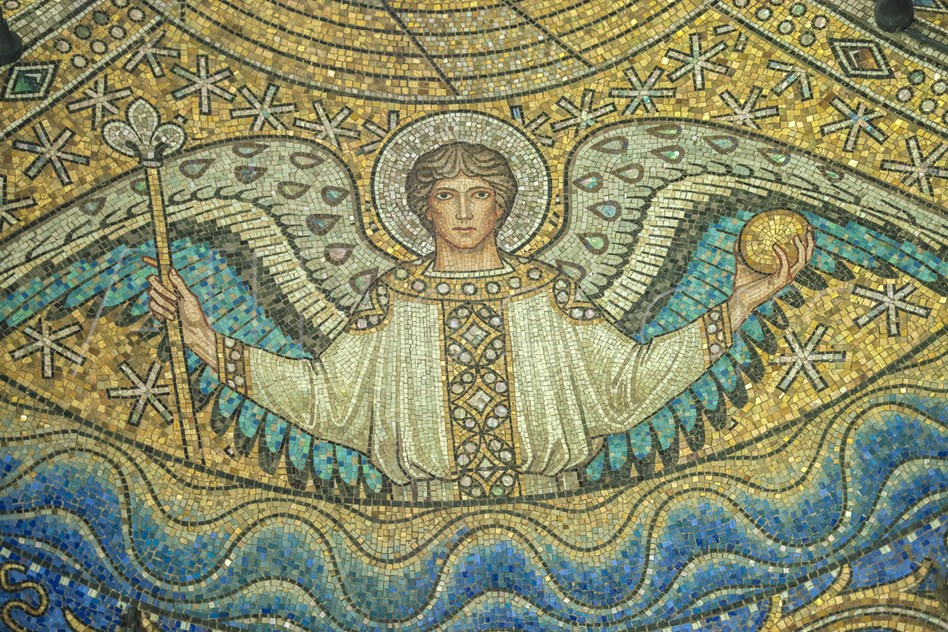
\includegraphics[width=6cm]{imagines/angelus.jpg}
\end{center}

\vfill

Fontes.
Textus et cantus officii divini secundum
Antiphonale Sacrosanctæ Romanæ Eclesiæ Pro Diurnis Horis, Romæ 1912
et Nocturnale Romanum, 2002, præter: psalmi 149 et 150 post
psalmum 148 in Laudibus additi secundum Antiphonale Monasticum pro Diurnis Horis,
Solesmis 1934; lectio sancti Evangelii et hymnus Te Decet Laus post ultimum
responsorium additi secundum ritum monasticum vetum; responsorium breve
in Laudibus et Vesperis additum secundum Antiphonale Monasticum. /
Textus et cantus missæ secundum
Graduale triplex, Solesmis 1979. /
Translatio capituli et lectionis sumpta est ex:
Jeruzalémská bible, Praha-Kostelní Vydří 2009. /
Translationes psalmorum ex
Hejčl Jan: Žaltář čili Kniha žalmů, Praha 1922. /
Neumæ super canto missæ de codicibus Cantatorium, Stiftsbibl. 359 et
Einsiedeln,
Stiftsbibl. 121 et neumæ super canto officii divini de codice Hartker,
Stiftsbibl. 391.

Collaborantes.
Textus latinos cantusque transcripsit et omnem laborem typographicum peregit
Jakub Jelínek. /
Proprios cantus festi in linguam bohemicam Václav Ondráček transtulit. /
Psalmos in lingua bohemica de libro supra dicto transcripsit
Barbora Maturová et idem Jakub Jelínek. /
Filip Srovnal librum istum præparare mandavit et laborem exprobrationibus
utilissimis comitabatur. Iste etiam librum totum ante publicationem
diligenter legit et plurimos errores invenit. /
Imaginem, quæ paginam tituli ornat, Klára Jirsová pinxit.

Instrumenta adhibita.
LuaTeX, %http://www.luatex.org / 
Gregorio, %http://home.gna.org/gregorio /
typi Junicode. %http://junicode.sourceforge.net

\begin{center}
Liber hic imprimis ad usum chori 
\guillemotright Conventus Choralis\guillemotleft\ 
paratus est
et secundum eius consuetudines.
http://www.introitus.cz

\vspace{1cm}

{\large Editio Sancti Wolfgangi 2015.}

\vspace{2mm}

Series \guillemotright Conventus\guillemotleft, vol. II.

\vspace{1cm}

http://stiwolfgangi.xf.cz

\vfill

\today

\end{center}

\end{document}
